\documentclass[10pt]{article}
\usepackage[left=2.54cm, right=2.54cm, top=2.54cm, bottom=2.54cm]{geometry}  % Márgenes
\usepackage{hyperref}
\hypersetup{breaklinks=true}
\usepackage[utf8]{inputenc}
\usepackage[T1]{fontenc}
\usepackage{lmodern}
\usepackage{geometry}
\usepackage{parskip}
\usepackage{graphicx}  % Para usar \scalebox
\usepackage{lettrine}
\usepackage{booktabs}
\usepackage{caption}
\usepackage{url}
\usepackage{microtype} % Mejora la justificación y reduce overfull hbox
\usepackage{amsmath}
\usepackage{placeins}
\usepackage{array}
\usepackage{siunitx}

\usepackage[utf8]{inputenc}
\usepackage[T1]{fontenc}
\usepackage{url}
\usepackage{hyperref}
\usepackage{float}
\usepackage{tabularx}
\usepackage{adjustbox}
\usepackage{threeparttable}
\usepackage{subcaption}
\usepackage{longtable} % Cargar el paquete longtable
\usepackage{ltablex} % Combina longtable y tabularx
\usepackage{xcolor}
\keepXColumns  

\sisetup{
  round-mode          = places,
  round-precision     = 2,
  table-number-alignment = center,
  detect-all
}
% Carga la definición de la fuente Goudy Initialen
\input GoudyIn.fd
% Define un comando para usar la fuente Goudy Initialen
\newcommand*\initfamily{\usefont{U}{GoudyIn}{xl}{n}}
% Definir comando \doi para formatear el DOI como enlace
\newcommand{\doi}[1]{\href{https://doi.org/#1}{doi:#1}}
\title{Customer Segmentation in Shopping Malls: Analysis and Marketing Strategies}
\author{Sebastián David Pinzón Zambrano \\ {\small Data Scientist}}
\date{}
\begin{document}
\maketitle

\begin{center}
    {\footnotesize \textbf{Resumen}}  
\end{center}

\begin{center}
    \begin{minipage}{0.85\textwidth} % Ajusta el ancho aquí (ej. 0.8 reduce los márgenes)
        {\footnotesize
        The study analyzes customer segmentation in shopping malls by means of the K-means algorithm, using a Kaggle dataset with demographic (age, gender, annual income) and behavioral (spending score) variables. After rigorous preprocessing (standardization and winsorization) and validation with indices such as the elbow method and the silhouette coefficient, six clusters were identified in a unisex analysis, highlighting young people with high income and high spending, while segmentation by gender revealed 11 clusters in men and 6 in women, with profiles such as young men with high spending and young women with high predisposition to consume despite low income. The results validate the usefulness of K-means for designing personalized marketing strategies, although limitations such as the size of the dataset and the absence of psychographic variables are pointed out, proposing future research with these variables and other algorithms to delve deeper into consumer behavior.
        }
    \end{minipage}
\end{center}

\vspace{10pt}
\section{Introduction}
\vspace{5pt}
\sloppy % Permite relajar la justificación y evitar overfull hbox

% Ejemplo con ajuste manual para 3 líneas
% Ajusta loversize y el escalado si es necesario
\lettrine[lines=3, loversize=0.01, lhang=0.01]{\scalebox{0.9}{\initfamily I}}{n} In the competitive retail environment, a deep understanding of customer characteristics and behaviors is essential to designing effective marketing strategies. The present research is based on a dataset provided by Kaggle, available at  \url{https://www.kaggle.com/datasets/vjchoudhary7/customer-segmentation-tutorial-in-python}, which includes demographic (age, gender, annual income) and shopping behavior (spending score) information of 200 customers of a shopping mall, obtained through membership cards. The variables analyzed include the customer's unique identifier, age, gender, annual income expressed in thousands of dollars, and a spending score assigned on a scale of 1 to 100, based on consumption patterns.

The main objective of this study is to profile customers, identifying those with the greatest buying potential, and to show that, even within the same gender, there are subgroups with differentiated behaviors. To achieve this, we use the K-means clustering algorithm, a robust unsupervised learning tool that segments the clientele into homogeneous and detailed profiles. This segmentation facilitates the detection of high-value customers, improves the understanding of diversity in consumption patterns and enables the formulation of personalized marketing strategies, thus optimizing resources in the management of the shopping center.

The analysis is developed at two levels: a global unisex approach and a specific segmentation by gender. In the global analysis, six optimal clusters are identified using a multimetric approach combining validation indices such as the elbow method, the silhouette coefficient, the Dunn index, the Calinski-Harabasz index and the Davies-Bouldin index. For men, 11 clusters are determined, reflecting greater heterogeneity, while for women 6 clusters are identified, indicating a greater concentration in consumption patterns. These segmentations are supported by advanced preprocessing techniques, including standardization to homogenize the scales of the variables and winsorization to treat outliers, ensuring the robustness of the results.

The findings reveal high-value segments, such as young men with high income and high spending, and young women with a high predisposition to consume despite low income. In addition, significant correlations are observed, such as an inverse relationship between age and expenditure in women (-0.4), absent in men, which underlines the relevance of considering gender in segmentation. These results not only enrich the understanding of purchase dynamics, but also provide a solid basis for the application of personalized marketing strategies in real retail environments.

Furthermore, the study pursues a dual purpose: to demonstrate the practical applicability of machine learning techniques in solving real-world problems and to serve as a methodological guide for researchers and practitioners interested in data science. Through a rigorous methodology and a detailed interpretation of emerging patterns, it seeks to provide a comprehensive view of consumer behavior, highlighting the importance of accurate segmentation that recognizes the inherent heterogeneity of the customer base.

Finally, although the project is developed in an academic and experimental context, the results lay a solid foundation for business applications. Accurate identification of profiles with high conversion probability, supported by multi-metric analysis and advanced techniques, can make a significant difference in competitiveness and business success, opening new perspectives for resource optimization and personalization in retail.

\section{State of the Art}
\vspace{10pt}
\lettrine[lines=3, loversize=0.01, lhang=0.01]{\scalebox{0.9}{\initfamily A}} review of the literature in the field of customer segmentation in shopping malls reveals a constant evolution in the application of quantitative and qualitative methodologies to understand consumer behavior. Several studies have approached this topic from multiple perspectives, offering a broad overview of the problems to be solved, the methodologies employed, the results obtained and the limitations encountered.

\subsection{Problems addressed in previous studies}

The analyzed scientific works have identified several key issues, such as:

\begin{itemize}
    \item \textbf{Understanding and defining customer segments:} Research such as Gilboa (2009) has focused on developing typologies that allow the identification of homogeneous groups based on behaviors and demographic characteristics. Similarly, recent studies have attempted to classify customers not only by their demographic data but also by integrating psychographic and behavioral variables (for example, “Mall Enthusiasts” or “Deal Hunters”), which is essential for directing personalized marketing strategies.
    
    \item \textbf{Adaptation to changing economic and technological contexts:} Some works have highlighted how changes in the economic environment, especially during periods of crisis, modify purchasing behavior. Studies focused on “profiling shopping mall customers during hard times” emphasize the need for dynamic segmentations that respond to the evolution of market conditions and digital transformation.
    
    \item \textbf{Limitations of traditional methods:} The literature shows that classical approaches based solely on demographic data or traditional clustering models (such as k-means) may lack interpretability or fail to fully capture the complexity of customer behaviors. This issue has motivated the integration of deep learning methods and explainable analysis (for example, through models like DeepLimeSEG) to improve both the accuracy and interpretation of the obtained segments.
\end{itemize}

\subsection{Methodologies and Applied Approaches}

The reviewed studies have used various techniques to address segmentation, among which the following stand out:

\begin{itemize}
    \item \textbf{Traditional clustering techniques:} Many authors have employed algorithms such as k-means and hierarchical clustering to identify segments based on variables such as age, annual income, and spending score. These methods allow for an initial classification of customers and have been used in both classical and recent research to delineate consumption profiles in shopping centers.
    
    \item \textbf{Integration of RFM analysis and advanced techniques:} The combination of RFM analysis (Recency, Frequency, and Monetary Value) with clustering algorithms has been recurrent, as it allows for capturing behavioral patterns more precisely. Some studies have complemented this methodology with association rules and conjoint analysis to identify product bundles and the specific preferences of each segment.
    
    \item \textbf{Application of deep learning and explainable models:} In view of the limitations of traditional methods, innovative approaches have been proposed that integrate neural networks with explainable artificial intelligence techniques (XAI). These models not only improve segmentation accuracy but also facilitate the interpretation of the key factors in purchasing behavior, providing a more robust framework for targeted marketing strategies.
    
    \item \textbf{Multi-method approaches and comparative analysis:} Several studies have opted to combine quantitative and qualitative methods to obtain a holistic view of the consumer. This includes the integration of statistical analyses (for example, ANOVA, regressions) with case studies and international comparisons, which enrich the understanding of cultural and contextual particularities in customer segmentation.
\end{itemize}

\subsection{Main Findings and Limitations}

Among the most relevant results, the following stand out:

\begin{itemize}
    \item \textbf{Identification of differentiated segments:} The literature has shown the existence of customer groups with very diverse behaviors and characteristics, ranging from those with a high propensity to spend and high purchasing power to segments with more moderate consumption patterns or those resistant to economic changes.
    
    \item \textbf{Importance of psychographic factors:} Recent studies emphasize that the incorporation of psychographic variables (attitudes, perceptions, and motivations) significantly improves the quality of segmentation, allowing for a classification that goes beyond demographics and better reflects consumer preferences.
    
    \item \textbf{Challenges in model interpretability and generalization:} Despite methodological advances, it is recognized that some approaches, especially those based on deep learning, may present difficulties in interpreting the results. Moreover, the generalization of the findings to different contexts and formats of shopping centers continues to be a challenge, which opens the door to future research to adapt and validate these models in varied environments.
\end{itemize}

\subsection{Connection with the Present Research}

In this context, the current research positions itself as an innovative contribution, since it:

\begin{itemize}
    \item Proposes the integration of advanced machine learning techniques and explainable methods for customer segmentation, seeking to overcome the limitations identified in previous studies.
    
    \item Provides a differentiated perspective by combining demographic and psychographic variables, which allows for generating a more robust and contextually adapted profile of potential customers in shopping centers.
    
    \item Focuses on validating the applicability of these methodologies in both academic and business environments, with the aim of providing practical tools that optimize marketing strategies in the sector.
\end{itemize}

This state of the art not only demonstrates a deep knowledge of the topic and the diversity of existing approaches, but also justifies the relevance and originality of the present study. It highlights the need to continue exploring integrated models that allow for obtaining more interpretable and generalizable segmentations, responding to current market demands and adding value to strategic decision-making.

\section{Methodology}
\lettrine[lines=3, loversize=0.01, lhang=0.01]{\scalebox{0.9}{\initfamily T}}{h}is section provides a detailed description of the methodological approach used to analyze and segment customer behavior. Starting with a dataset obtained from Kaggle, which includes demographic and spending variables, the process begins with rigorous preprocessing: cleaning the data, identifying and treating outliers through winsorization, and standardizing to ensure the integrity and homogeneity of the information.

Subsequently, an exploratory analysis is performed to identify key patterns and relationships among the variables, supported by visualization techniques and statistical validation. The determination of the optimal number of clusters is carried out by integrating various validation indices---such as the elbow method, silhouette coefficient, Dunn index, Calinski-Harabasz, and Davies-Bouldin indices---ensuring robust segmentation.

Finally, the KMeans algorithm is implemented to group customers into homogeneous segments, facilitating the identification of profiles with high conversion potential and providing a solid foundation for applying personalized marketing strategies and machine learning techniques in real-world commercial environments.

\subsection{Dataset}
\sloppy
The present study is based on the analysis of a dataset obtained from Kaggle, which is available at the following link: \url{https://www.kaggle.com/datasets/vjchoudhary7/customer-segmentation-tutorial-in-python}. This dataset consists of 200 observations and 5 variables: \texttt{CustomerID}, \texttt{Age}, \texttt{Annual Income (k\$)}, and \texttt{Spending Score (1-100)}.

The structure of the dataset is described in Table~\ref{tab:columnas}, which details the name of each variable, its data type, and its respective explanation. This resource has been developed for educational and experimental purposes, aimed at teaching customer segmentation techniques and market analysis using the KMeans clustering algorithm. Although it is assumed that the data comes from a real environment, likely a shopping mall or supermarket, specific details such as the collection date or exact location are not provided.

The dataset is shared through a GitHub repository, which highlights its educational purpose and the intention to provide researchers and students with a practical tool for applying machine learning methods in customer segmentation.

\begin{table}[h]
    \centering
    \caption{Column Format, Data Types, and Explanations}
    \begin{tabular}{ll>{\raggedright\arraybackslash}p{7cm}}
        \toprule
        \textbf{Column} & \textbf{Data Type} & \textbf{Explanation} \\
        \midrule
        CustomerID             & int64   & Unique identifier assigned to each customer. \\
        Gender                 & object  & Customer's gender. \\
        Age                    & int64   & Customer's age. \\
        Annual Income (k\$)    & int64   & Customer's annual income, expressed in thousands of dollars. \\
        Spending Score (1-100) & int64   & Score assigned by the shopping center based on the customer’s spending behavior and pattern. \\
        \bottomrule
    \end{tabular}
    \label{tab:columnas}
\end{table}

\subsection{Preprocessing}

Data preprocessing is a fundamental stage in any analysis, as it ensures that the information to be used is of the highest quality and free from errors. In this process, techniques using \texttt{pandas} were implemented to identify and remove erratic data and outliers, such as \texttt{NaN}, \texttt{inf}, \texttt{-inf}, and completely empty rows. In our case, no inconsistencies or empty rows were detected, so the dataset remained intact.

Below is a comparison of the dataset's status before and after preprocessing (see Table~\ref{tab:estado_datos}):

\begin{table}[h]
    \centering
    \caption{Comparison of Data Status}
    \label{tab:estado_datos}
    \begin{tabular}{lcc}
        \toprule
        \textbf{Status} & \textbf{Rows} & \textbf{Columns} \\
        \midrule
        Before   & 200 & 5 \\
        After & 200 & 5 \\
        \bottomrule
    \end{tabular}
\end{table}

Subsequently, a detailed analysis was conducted to detect outliers in the \texttt{Annual Income (k\$)}, \texttt{Age}, and \texttt{Spending Score (0-100)} columns. The distribution of these data was explored using a histogram and a boxplot, providing a comprehensive understanding of their behavior (see Figure~\ref{fig:miGrafico}).

The analysis identified and removed two outlier values present in the \texttt{Annual Income (k\$)} column. It is important to note that no outliers were found in the \texttt{Age} and \texttt{Spending Score (0-100)} columns. A summary of this process is detailed in Table~\ref{tab:outliers_eliminate}.
\begin{figure}[h]
    \centering
    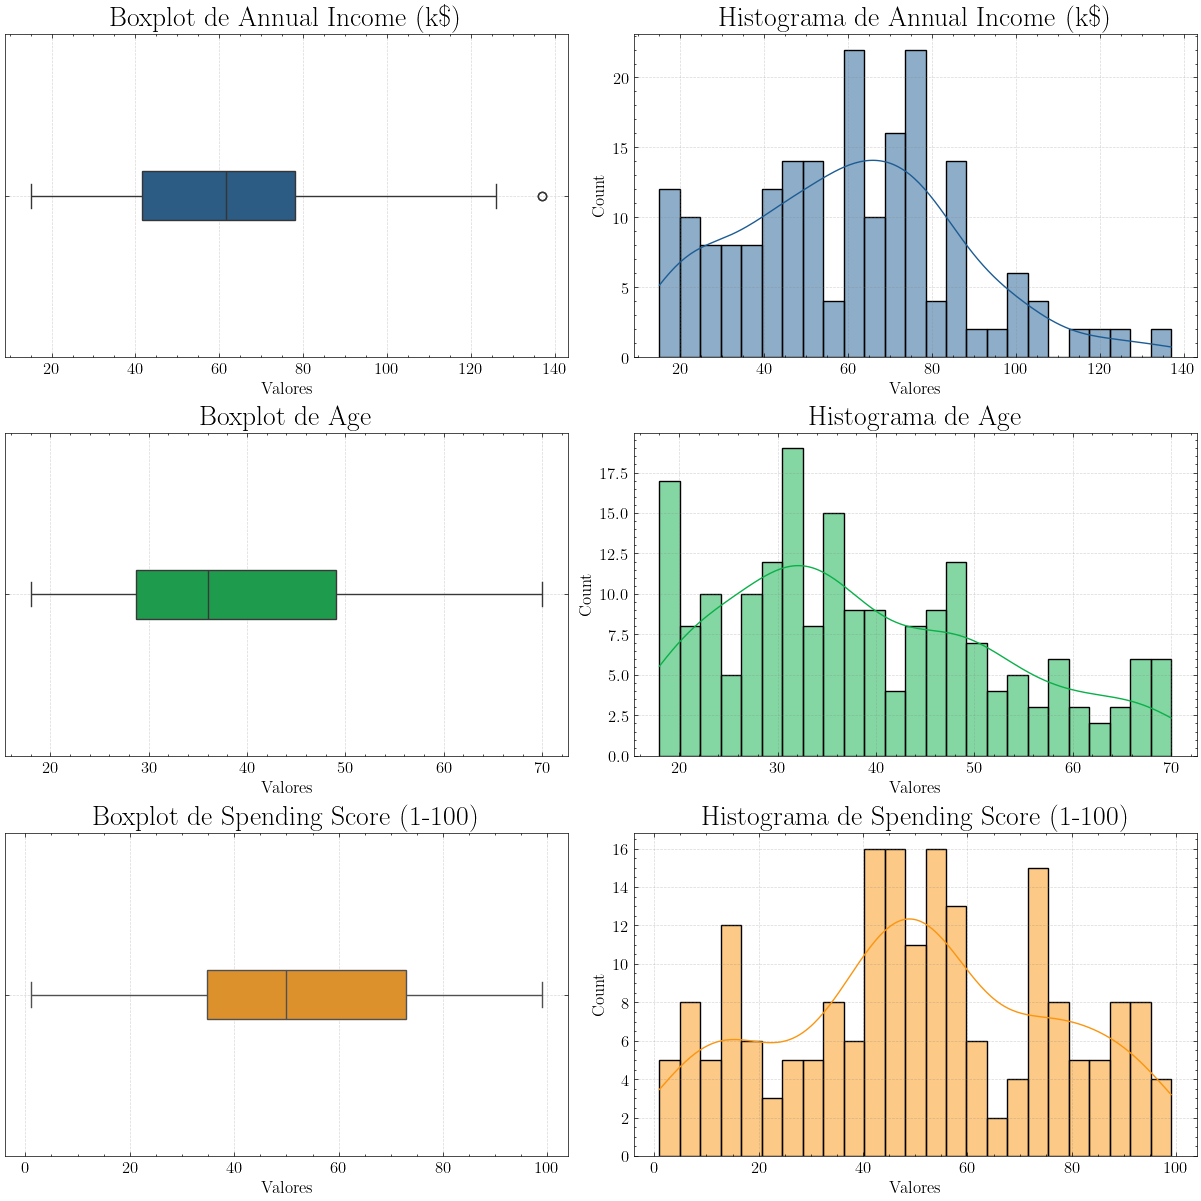
\includegraphics[width=0.8\textwidth]{plots_investing/Grafico 1.png}
    \caption{Data distribution represented through a histogram and a boxplot.}
    \label{fig:miGrafico}
\end{figure}

\begin{table}[h]
    \centering
    \caption{Eliminated Outliers}
    \label{tab:outliers_eliminate}
    \begin{tabular}{lr}
    \hline
    \textbf{Column} & \textbf{Number of Outliers} \\
    \hline
    Annual Income (k\$)        & 2 \\
    Age                       & 0 \\
    Spending Score (0-100)    & 0 \\
    Total rows eliminated & 2 \\
    \hline
    \end{tabular}
\end{table}

Finally, after an exhaustive process of data cleaning and analysis, standardization was performed using the \texttt{StandardScaler} technique. This procedure ensures that all variables are on the same scale, which not only facilitates subsequent analysis but also optimizes the performance of the customer segmentation models. In this way, a rigorous and consistent treatment of the data is ensured, laying the groundwork for future studies and analyses with a high level of precision and reliability.

Additionally, a comparative analysis of the modifications applied to the \texttt{Age}, \texttt{Annual Income (k\$)}, \texttt{Spending Score (0-100)}, and \texttt{Gender} variables was performed. Through detailed visualization, the changes experienced by these variables before and after standardization are illustrated, providing a clear representation of the impact of this process on the data structure (see Figure~\ref{fig:miGrafico2}).

\begin{figure}[p]
    \centering
    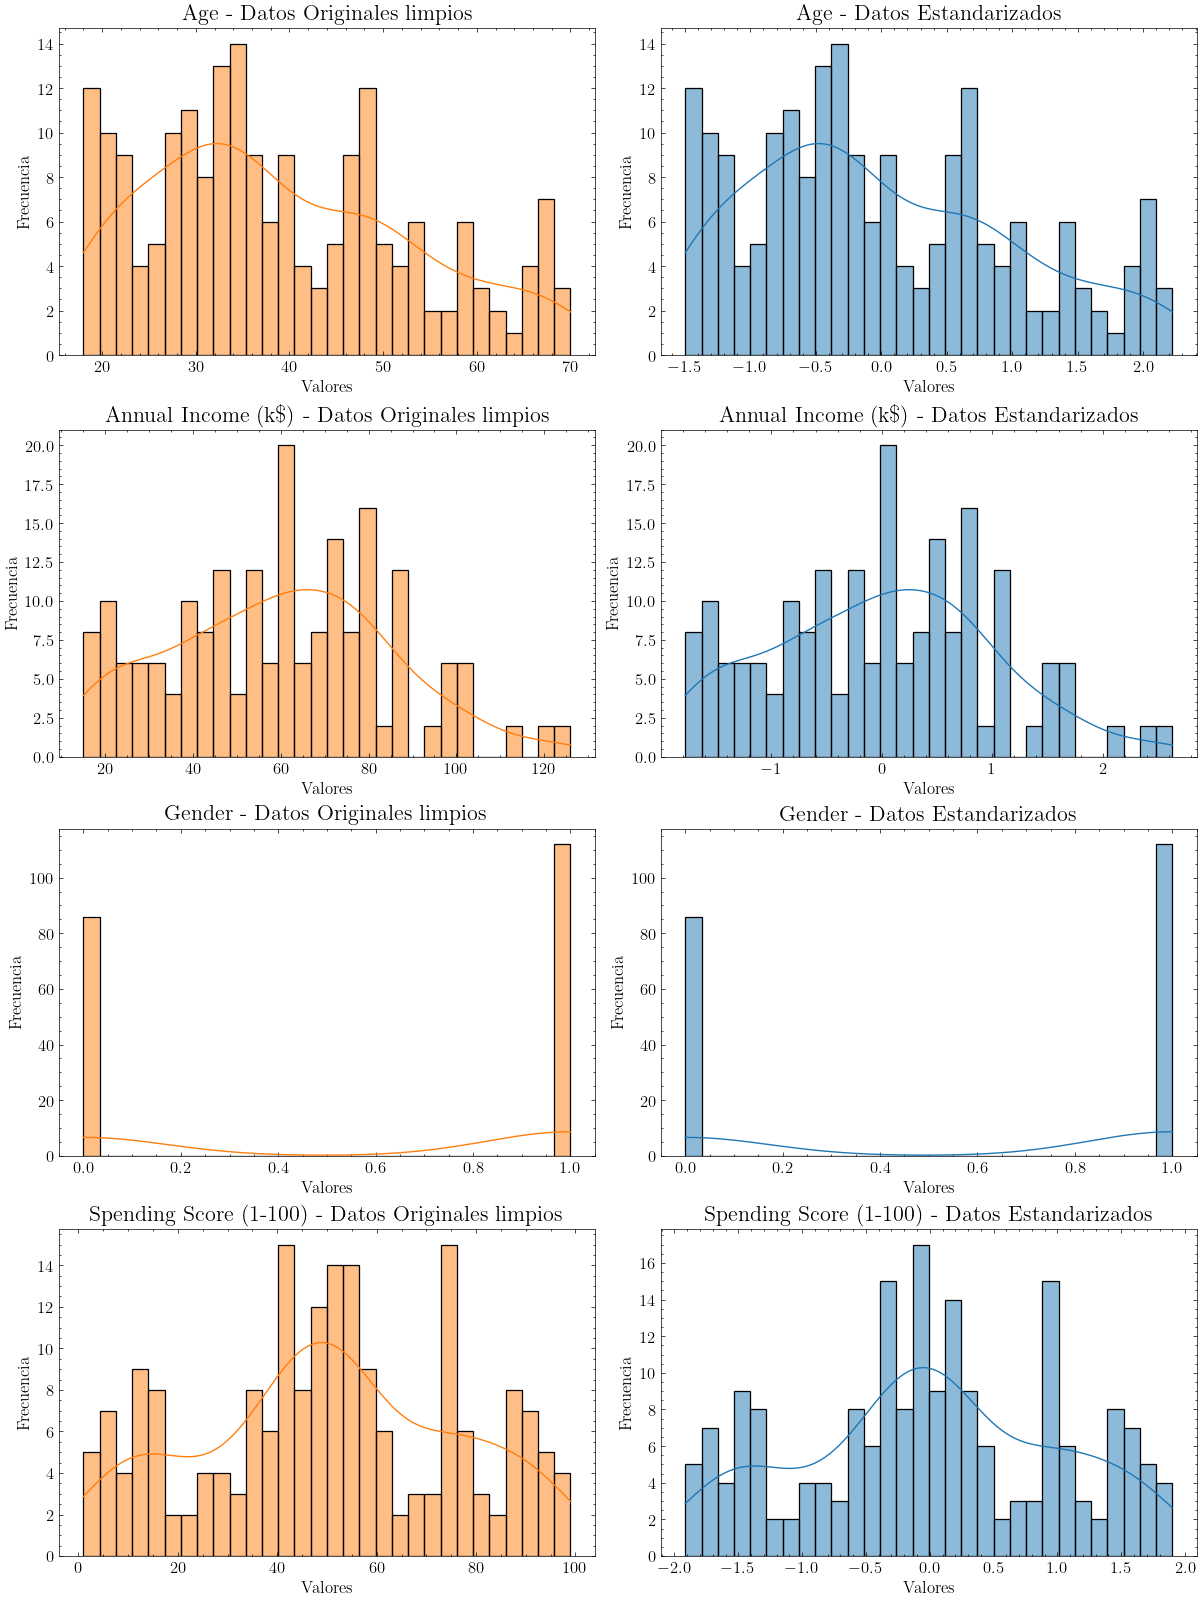
\includegraphics[width=0.8\textwidth]{plots_investing/Grafico 2.png}
    \caption{Comparative visualization of data before and after standardization.}
    \label{fig:miGrafico2}
\end{figure}



\subsection{Exploratory Analysis}

We will begin exploring the data using a correlation map or "Heatmap" as an initial tool. This instrument will allow us to identify significant correlations that could reveal patterns not immediately evident, as well as help us avoid collinearity issues among variables.

\begin{figure}[h]
    \centering
    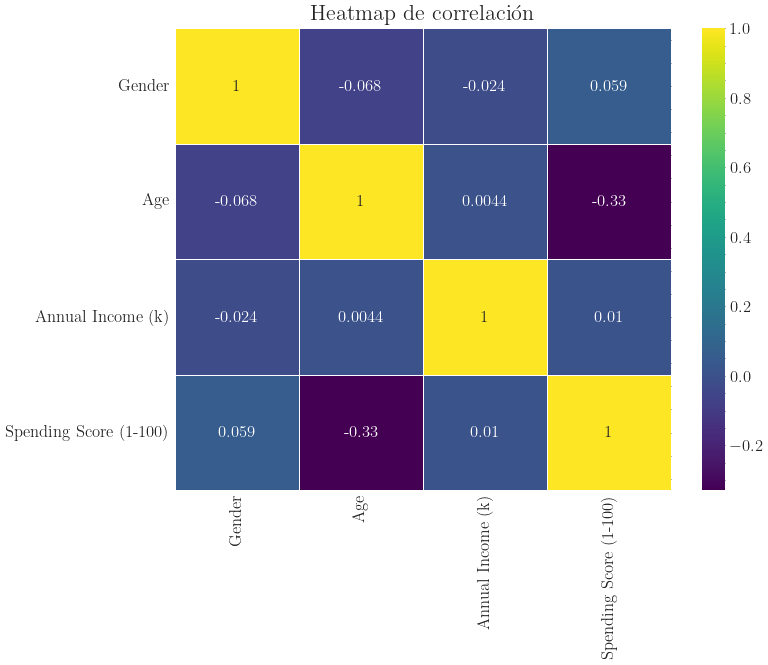
\includegraphics[width=0.8\textwidth]{plots_investing/Grafico 3.png}
    \caption{Visualization of the heatmap for the analysis of correlations among variables.}
    \label{fig:miGrafico3}
\end{figure}

Figure \ref{fig:miGrafico3} presents the resulting heatmap. Through this analysis, no collinearity problems were detected among the studied variables. However, a negative correlation between "Age" and "Spending Score (0-100)" is notable. Although this correlation is relatively weak, it suggests that as a customer's age increases, their spending score tends to decrease.

It is important to note that this study is conducted on the entire sample, including both men and women, so the exploratory analysis considers the complete dataset.

To examine this hypothesis in greater detail, we calculated the average Spending Score for each age group, which allows us to visualize the spending pattern in relation to the consumer's age. In this analysis, we implemented a linear regression to determine the overall trend of the relationship, complemented with a LOWESS (Locally Weighted Scatterplot Smoothing) smoother to reduce noise in the data.

Once the LOWESS smoothing was applied, we complemented our analysis with a histogram that represents the percentage change relative to the previous point, calculated from the smoothed values. This approach allows us to identify trend changes more clearly, as shown in Figure \ref{fig:miGrafico4}.

\begin{figure}[h]
    \centering
    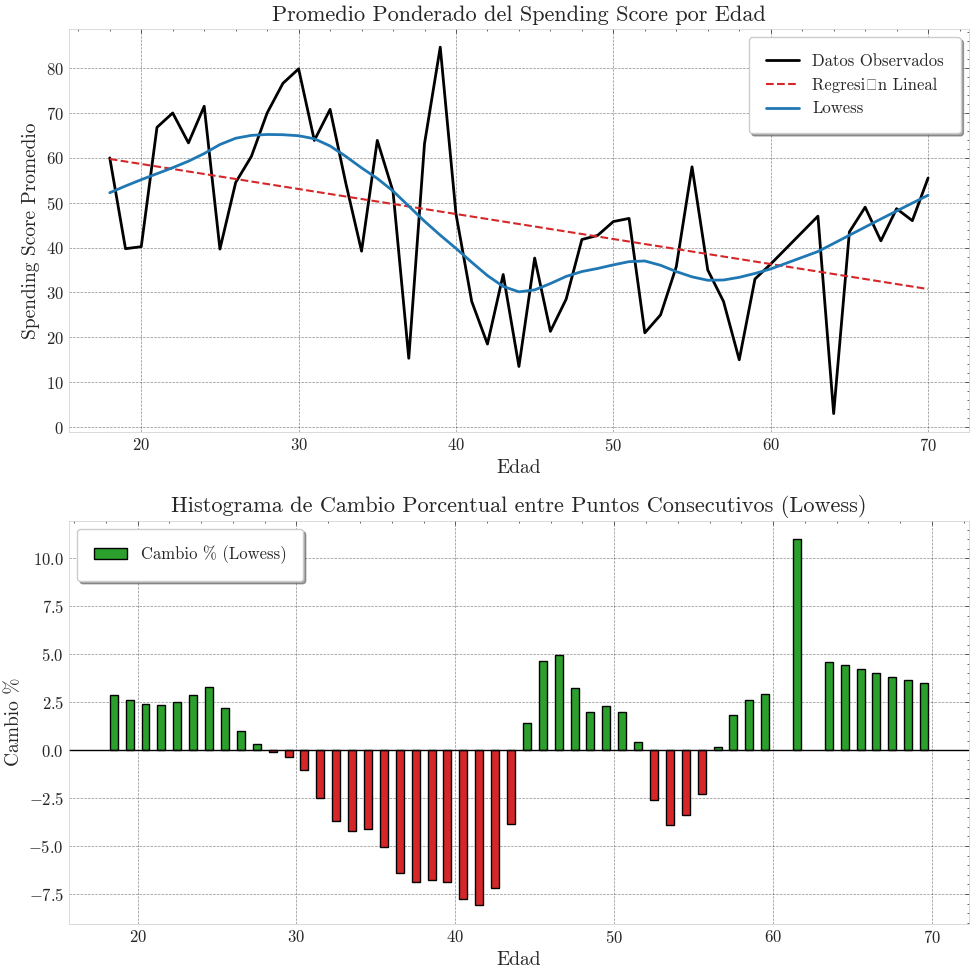
\includegraphics[width=0.8\textwidth]{plots_investing/Grafico 4.png}
    \caption{Variation of the Spending Score by age with LOWESS smoothing and percentage change histogram.}
    \label{fig:miGrafico4}
\end{figure}

The initial hypothesis suggesting an inversely proportional relationship between age and spending is supported by the overall trend observed in the linear regression. However, when examining the data from a fractal perspective, the percentage change histogram reveals that this relationship is not uniform across the entire age spectrum. On the contrary, segments with both positive and negative trends are identified.

These trend ranges allow us to segment the age spectrum and draw conclusions about the age groups with the highest potential as customers, as summarized in Table \ref{tab:spending_score}.

\begin{table}[H]
    \centering
    \sisetup{table-format=2.2} % Configuration to align numbers in column
    \renewcommand{\arraystretch}{1.2} % Row spacing
    \caption{Spending Score Trend by Age Range}
    \label{tab:spending_score}
    \begin{tabular}{llS}
        \toprule
        \textbf{Trend} & \textbf{Age Range} & \textbf{Weighted Average Spending Score} \\
        \midrule
        Upward & 18.0 -- 29.0 & 59.39 \\
        Downward & 28.0 -- 45.0 & 50.74 \\
        Upward & 44.0 -- 53.0 & 32.38 \\
        Downward & 52.0 -- 57.0 & 33.79 \\
        Upward & 56.0 -- 70.0 & 37.04 \\
        \bottomrule
    \end{tabular}
\end{table}

From this initial exploration, we can infer that, despite the complexity revealed by the fractal analysis, there is clear evidence of age-related patterns in spending behavior. If the goal is to optimize resources by focusing on segments with a higher potential to convert into frequent customers, the data suggests prioritizing the age range between 18 and 29, while not neglecting the segment between 28 and 45. The recommended strategy would be to diversify the product offerings targeted at these age groups.

Regarding the age segment between 45 and 70, which exhibits a significantly lower spending behavior, a deeper study would be required to determine the underlying causes of this trend. However, such an analysis is beyond the scope of the present study due to the limitations of the available dataset.

This is only a preliminary observation; now we will proceed to use the K-means technique to uncover patterns in the dataset.


\subsubsection{Global Unisex Study}

Initially, we will examine the three-dimensional distribution of the data using the variables “Annual Income (k\$)”, “Age”, and “Spending Score (1-100)”. The exclusion of the “Gender” variable is aligned with our goal of conducting an integrated analysis without gender distinction, which will allow us to identify universal patterns in customer behavior. Including this variable would not only be unnecessary but would also add additional complexity without substantial analytical benefit.

\begin{figure}[h]
    \centering
    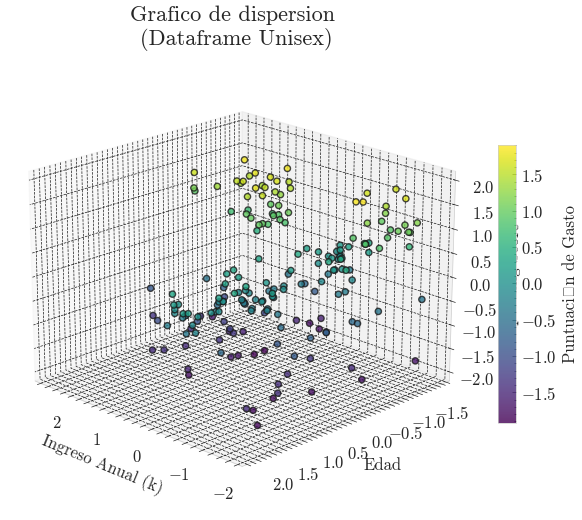
\includegraphics[width=0.8\textwidth]{plots_investing/Grafico 5.png}
    \caption{Three-dimensional visualization of the data distribution according to annual income, age, and spending score.}
    \label{fig:miGrafico5}
\end{figure}

Figure \ref{fig:miGrafico5} shows the three-dimensional distribution of the analyzed dataset.

Prior to applying the K-means algorithm, it is essential to determine the optimal number of clusters that best represent the intrinsic structure of the data.

The scientific literature offers various methodologies for determining the optimal number of clusters. In this study, we have chosen a comprehensive approach that combines five validation indices, each with complementary strengths. This multimetrical approach, in addition to providing a holistic view, allows us to avoid tie situations by using an odd number of indicators.

\begin{figure}[p]
    \centering
    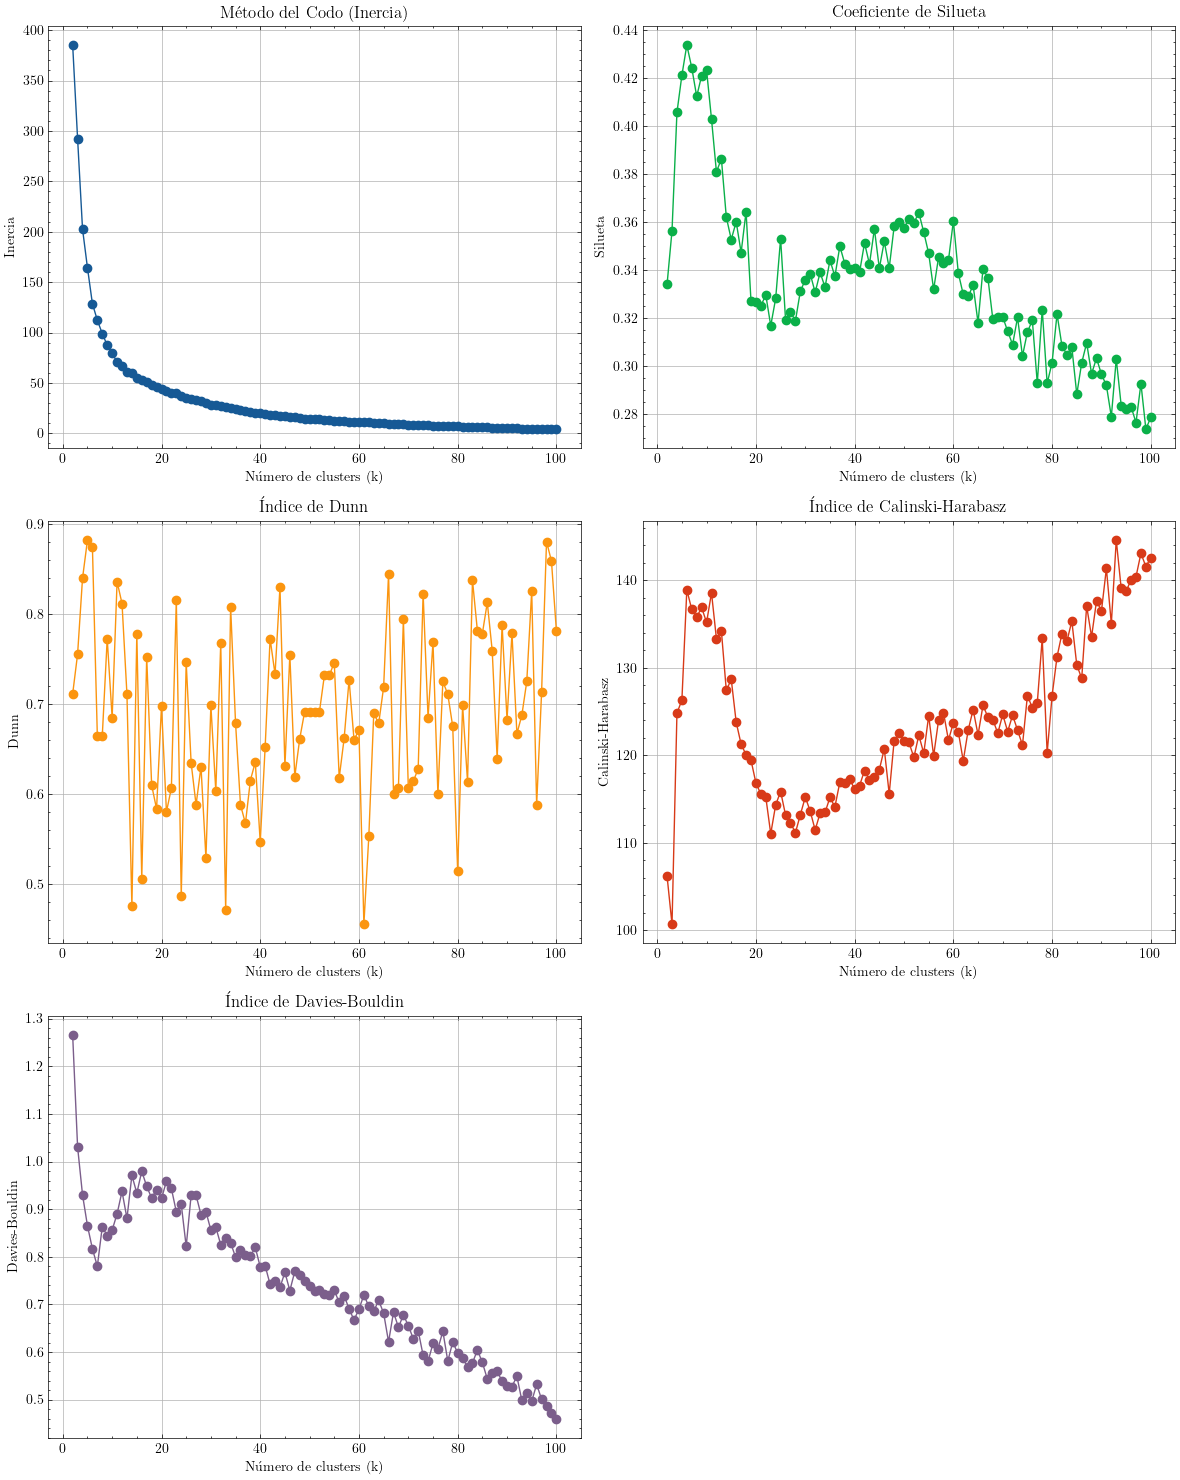
\includegraphics[width=0.8\textwidth]{plots_investing/Grafico 6.png}
    \caption{Evolution of the cluster validation indices as a function of the number of groupings.}
    \label{fig:miGrafico6}
\end{figure}

Figure \ref{fig:miGrafico6} presents the evolution of the five validation indices as a function of the number of clusters. It is important to note that an iterative analysis was performed, evaluating from 2 up to 101 clusters to obtain a complete perspective of the indices’ behavior.

The indices used were: the elbow method (Inertia), the Silhouette Coefficient, the Dunn Index, the Calinski-Harabasz Index, and the Davies-Bouldin Index.

To delimit the search area for optimal clusters, the elbow index was used to identify the starting point from the inflection of its curve, which indicated that the optimal initial value was \( k = 4 \).

Subsequently, the search range was extended up to \( k = 15 \). The endpoint of this area was determined by the convergence observed in the following indices:
\begin{itemize}
    \item \textbf{Dunn Index.}
    \item \textbf{Calinski-Harabasz Index.}
    \item \textbf{Davies-Bouldin Index.}
\end{itemize}

With the increase in \( k \), a marked drawdown was observed in these indicators, which allowed defining \( k = 15 \) as the upper limit of the area of interest.

It is important to clarify that this procedure was based on a visual and intuitive interpretation of the graphs, and not on a rigorous statistical calculation.

\begin{figure}[h]
    \centering
    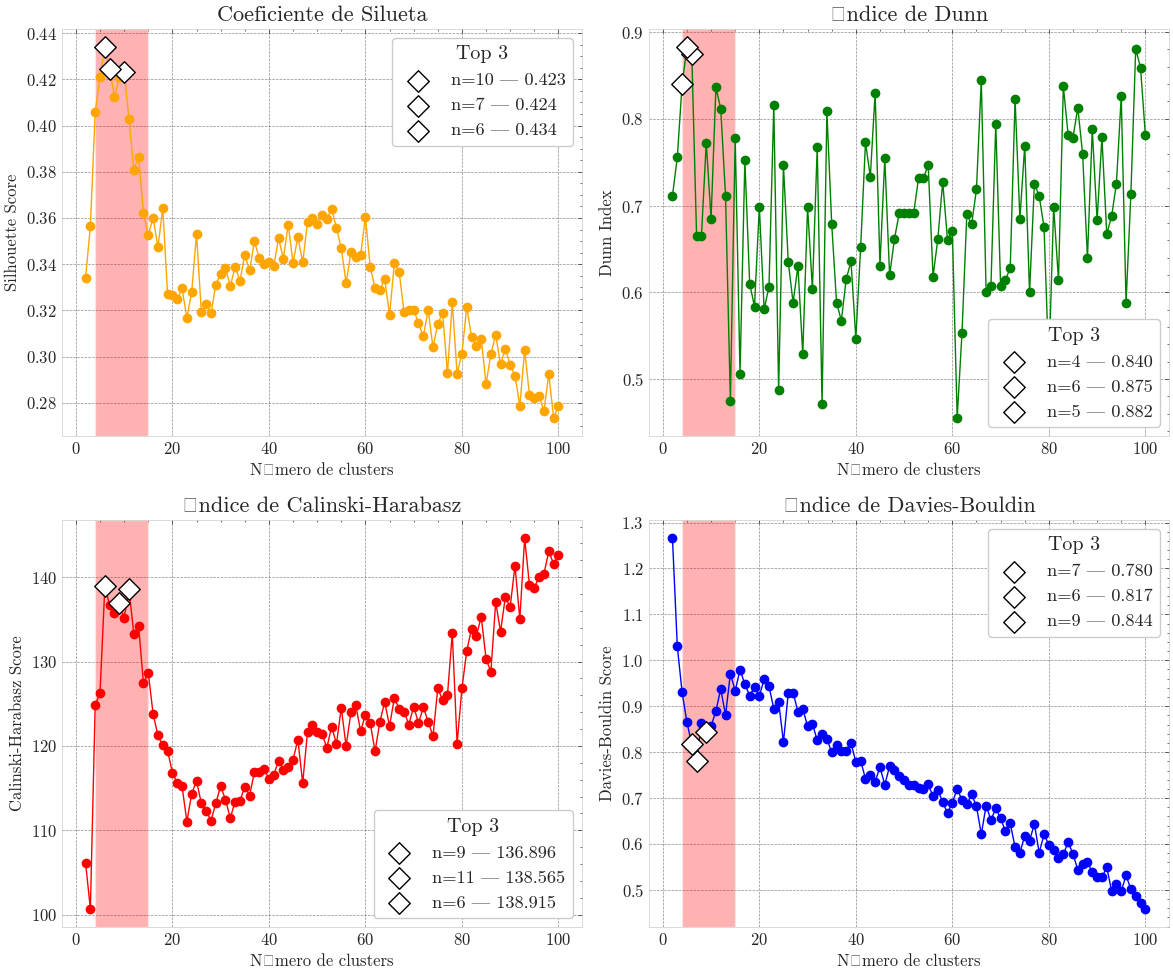
\includegraphics[width=0.8\textwidth]{plots_investing/Grafico 7.png}
    \caption{Identification of optimal values for each validation index in the area of interest.}
    \label{fig:miGrafico7}
\end{figure}

Figure \ref{fig:miGrafico7} illustrates this refined analysis. Table \ref{tab:clusters_optimos} summarizes the results obtained for each metric, presenting the three optimal clusters identified by each index.


\begin{table}[h]
    \centering
    \caption{\textbf{Optimal Clusters by Metric}}
    \label{tab:clusters_optimos}
    \renewcommand{\arraystretch}{1.2}
    \begin{tabular}{@{}lccc@{}}
        \toprule
        \textbf{Metric}         & \textbf{Optimal Cluster 1} & \textbf{Optimal Cluster 2} & \textbf{Optimal Cluster 3} \\
        \midrule
        Silhouette Coefficient  & 6                        & 7                        & 10                       \\
        Dunn Index              & 4                        & 5                        & 6                        \\
        Calinski-Harabasz       & 6                        & 9                        & 11                       \\
        Davies-Bouldin          & 6                        & 7                        & 9                        \\
        \bottomrule
    \end{tabular}
\end{table}

The convergence analysis of the obtained results suggests that the optimal number of clusters for the dataset is six (\( k = 6 \)). Once this value was determined, the \( k \)-means algorithm was implemented.

\begin{figure}[h]
    \centering
    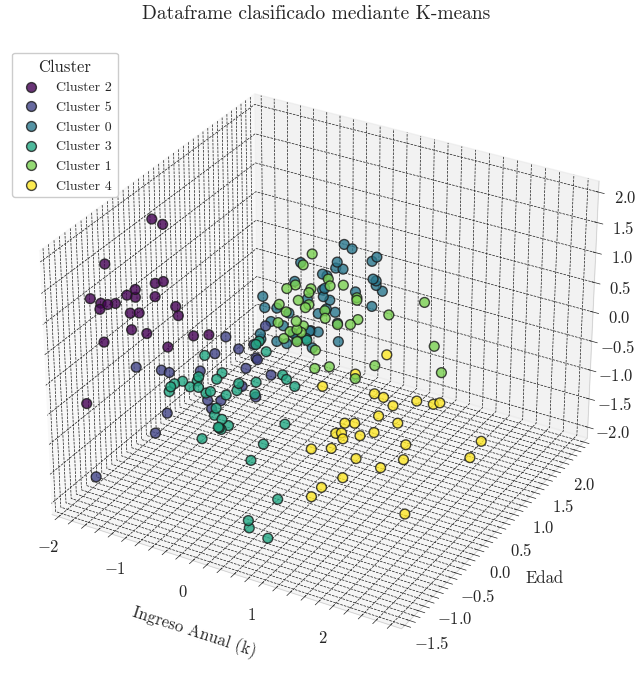
\includegraphics[width=0.8\textwidth]{plots_investing/Grafico 8.png}
    \caption{Visualization of the data classification into six clusters using the \( k \)-means algorithm.}
    \label{fig:miGrafico8}
\end{figure}

Figure~\ref{fig:miGrafico8} shows the resulting classification of the data into the six identified clusters.

To precisely characterize each cluster, a descriptive statistical analysis was developed covering measures of central tendency, such as the mean and median, as well as the standard deviation. In addition, the skewness coefficient was included to assess the symmetry of the data distribution in each grouping.

The inclusion of the skewness analysis is based on several methodologically significant considerations, allowing for a more complete and robust interpretation of the clusters' structure.

\begin{table}[h]
    \centering
    \caption{Statistics by Unisex Cluster}
    \label{tab:estadisticas_cluster}
    \resizebox{\textwidth}{!}{%
        \begin{tabular}{c%
                        S[table-format=2.2] S[table-format=2.2] S[table-format=2.2]%
                        S[table-format=2.2] S[table-format=2.2] S[table-format=2.2]%
                        S[table-format=2.2] S[table-format=2.2] S[table-format=2.2]%
                        S[table-format=1.2] S[table-format=2.2] S[table-format=2.2]}
            \toprule
            \multicolumn{1}{c}{Cluster} &
            \multicolumn{3}{c}{Age} &
            \multicolumn{3}{c}{Annual Income (k\$)} &
            \multicolumn{3}{c}{Spend Score} &
            \multicolumn{1}{c}{Age (skew)} &
            \multicolumn{1}{c}{Income (skew)} &
            \multicolumn{1}{c}{Spend Score (skew)} \\
            \cmidrule(lr){2-4} \cmidrule(lr){5-7} \cmidrule(lr){8-10}
             & {mean} & {std} & {median} &
               {mean} & {std} & {median} &
               {mean} & {std} & {median} &
               {skew} & {skew} & {skew} \\
            \midrule
            0 & 56.34 & 8.55 & 54.00 & 53.70 & 8.24 & 54.00 & 49.39 & 5.99 & 49.00 & 0.27 & -0.06 & -0.02 \\
            \textbf{1} & \textbf{32.76} & \textbf{3.75} & \textbf{32.00} & \textbf{85.21} & \textbf{14.24} & \textbf{78.50} & \textbf{82.11} & \textbf{9.49} & \textbf{84.00} & \textbf{0.38} & \textbf{1.23} & \textbf{-0.10} \\
            2 & 25.56 & 5.44 & 24.00 & 26.48 & 8.53  & 25.00 & 76.24 & 13.56 & 76.00 & 0.56 & 0.30  & -0.52 \\
            \textbf{3} & \textbf{26.12} & \textbf{7.03} & \textbf{25.00} & \textbf{59.42} & \textbf{10.59} & \textbf{60.00} & \textbf{44.45} & \textbf{14.28} & \textbf{48.00} & \textbf{0.71} & \textbf{-0.12} & \textbf{-1.65} \\
            \textbf{4} & \textbf{44.80} & \textbf{8.04} & \textbf{44.00} & \textbf{88.20} & \textbf{14.52} & \textbf{86.50} & \textbf{18.50} & \textbf{10.37} & \textbf{16.50} & \textbf{0.33} & \textbf{1.00}  & \textbf{0.31} \\
            5 & 45.52 & 11.77 & 46.00 & 26.29 & 7.44  & 25.00 & 19.38 & 12.56 & 15.00 & -0.08 & 0.34  & 0.17 \\
            \bottomrule
        \end{tabular}%
    }
\end{table}

The detailed results of this statistical characterization of the clusters are presented in Table~\ref{tab:estadisticas_cluster}, offering a comprehensive view of the distinctive properties of each grouping identified by the \( k \)-means algorithm.

As can be seen, there are inconsistencies in the skewness values in clusters 1, 3, and 4, since these values exceed the threshold of 0.7 or fall below the threshold of -0.7, which could indicate asymmetric distributions.

Since skewness is a factor that can affect the quality of the analysis, and considering that eliminating these data would be methodologically inappropriate, the winsorization technique was applied to adjust the outlier values. Figure~\ref{fig:miGrafico9} illustrates the comparison between the original data and those modified after applying winsorization.

\begin{figure}[h]
    \centering
    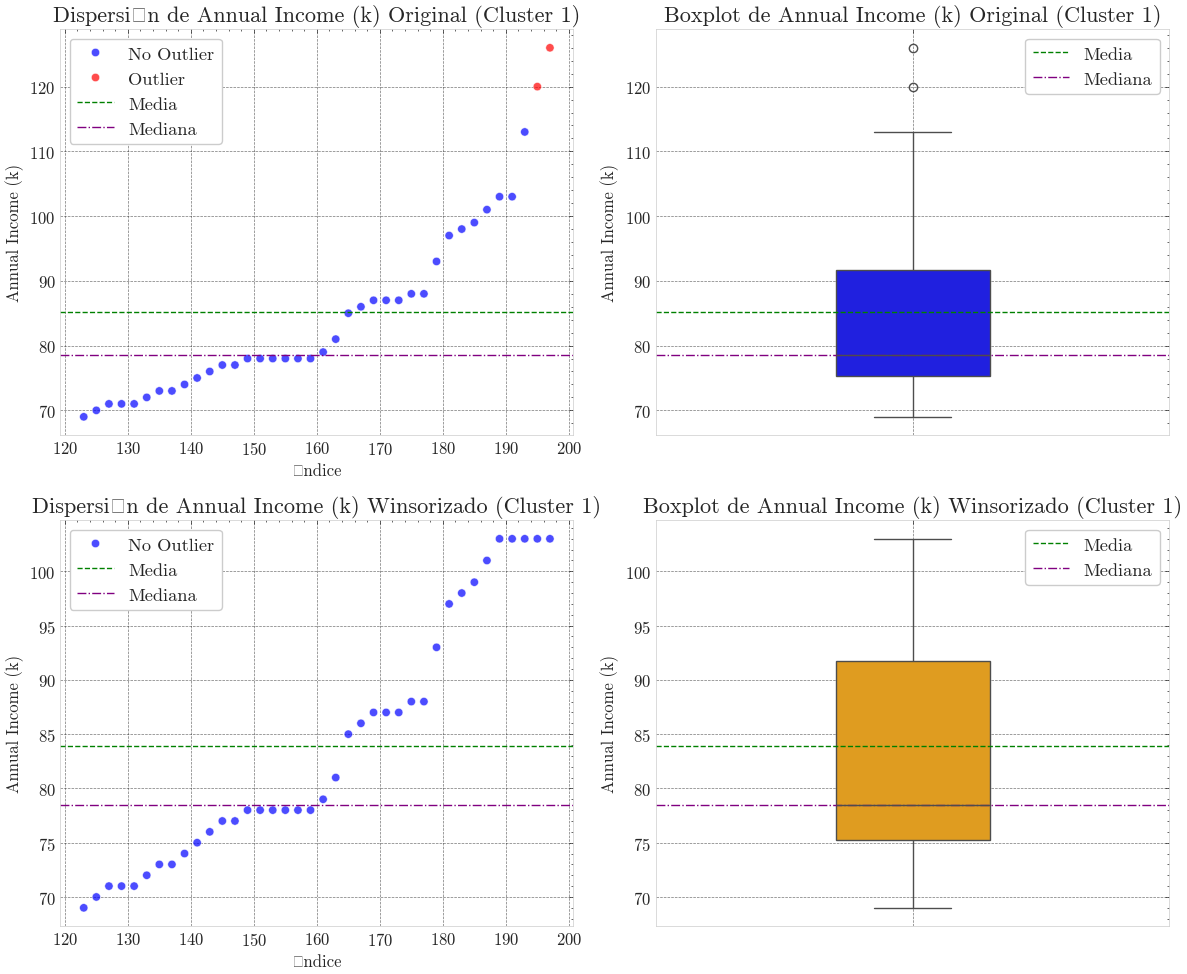
\includegraphics[width=0.8\textwidth]{plots_investing/Grafico 9.png}
    \caption{Comparison of distributions before and after winsorization.}
    \label{fig:miGrafico9}
\end{figure}

\begin{table}[h]
    \centering
    \caption{Summary of Transformations Applied to Each Cluster and Variable}
    \label{tab:procesamiento_clusters}
    \resizebox{\textwidth}{!}{%
    \begin{tabular}{ccccp{7cm}}
        \toprule
        \textbf{Cluster} & \textbf{Variable} & \textbf{Winsorization} & \textbf{IQR Factor} & \textbf{Change Description} \\
        \midrule
        1 & Annual Income (k) & [0, 0.1] & 1.5 & The top 10\% of extreme values was removed and outliers were detected with an IQR factor of 1.5 (Cluster 1). \\
        3 & Spending Score (1-100) & [0.1, 0] & 1.5 & The bottom 10\% of extreme values was removed and outliers were detected with an IQR factor of 1.5 (Cluster 3). \\
        3 & Age & [0, 0.2] & 0.5 & The top 20\% of extreme values was removed and outliers were detected with an IQR factor of 0.5 (Cluster 3). \\
        4 & Annual Income (k) & [0, 0.1] & 1.0 & The top 10\% of extreme values was removed and outliers were detected with an IQR factor of 1 (Cluster 4). \\
        \bottomrule
    \end{tabular}
    }
\end{table}

Table \ref{tab:procesamiento_clusters} details the transformations applied to each cluster and variable. As can be seen, winsorization and outlier detection were employed to correct the identified asymmetries. Table \ref{tab:estadisticas_winsor} shows the statistical results after applying these transformations.


\begin{table}[h]
    \centering
    \caption{Statistics by Unisex Cluster (after Winsorization)}
    \label{tab:estadisticas_winsor}
    \resizebox{\textwidth}{!}{%
        \begin{tabular}{c%
                        S[table-format=2.2] S[table-format=2.2] S[table-format=2.2]%
                        S[table-format=2.2] S[table-format=2.2] S[table-format=2.2]%
                        S[table-format=2.2] S[table-format=2.2] S[table-format=2.2]%
                        S[table-format=1.2] S[table-format=2.2] S[table-format=2.2]}
            \toprule
            \multicolumn{1}{c}{Cluster} &
            \multicolumn{3}{c}{Age} &
            \multicolumn{3}{c}{Annual Income (k\$)} &
            \multicolumn{3}{c}{Spend Score} &
            \multicolumn{1}{c}{Age (skew)} &
            \multicolumn{1}{c}{Income (skew)} &
            \multicolumn{1}{c}{Spend Score (skew)} \\
            \cmidrule(lr){2-4} \cmidrule(lr){5-7} \cmidrule(lr){8-10}
             & {mean} & {std} & {median} &
               {mean} & {std} & {median} &
               {mean} & {std} & {median} &
               {skew} & {skew} & {skew} \\
            \midrule
            0 & 56.34 & 8.55 & 54.00 & 53.70 & 8.24 & 54.00 & 49.39 & 5.99 & 49.00 & 0.27 & -0.06 & -0.02 \\
            1 & 32.76 & 3.75 & 32.00 & 83.89 & 11.31 & 78.50 & 82.11 & 9.49 & 84.00 & 0.38 & 0.56  & -0.10 \\
            2 & 25.56 & 5.44 & 24.00 & 26.48 & 8.53 & 25.00 & 76.24 & 13.56 & 76.00 & 0.56 & 0.30  & -0.52 \\
            3 & 25.02 & 5.21 & 25.00 & 59.42 & 10.59 & 60.00 & 46.55 & 9.31 & 48.00 & 0.11 & -0.12 & -0.56 \\
            4 & 44.80 & 8.04 & 44.00 & 86.53 & 11.20 & 86.50 & 18.50 & 10.37 & 16.50 & 0.33 & 0.26  & 0.31 \\
            5 & 45.52 & 11.77 & 46.00 & 26.29 & 7.44 & 25.00 & 19.38 & 12.56 & 15.00 & -0.08 & 0.34  & 0.17 \\
            \bottomrule
        \end{tabular}%
    }
\end{table}

With the data now transformed and presenting more appropriate skewness indices, we proceeded to generate a heatmap for each cluster to identify any additional patterns, as shown in Figure \ref{fig:miGrafico10}.

\begin{figure}[h]
    \centering
    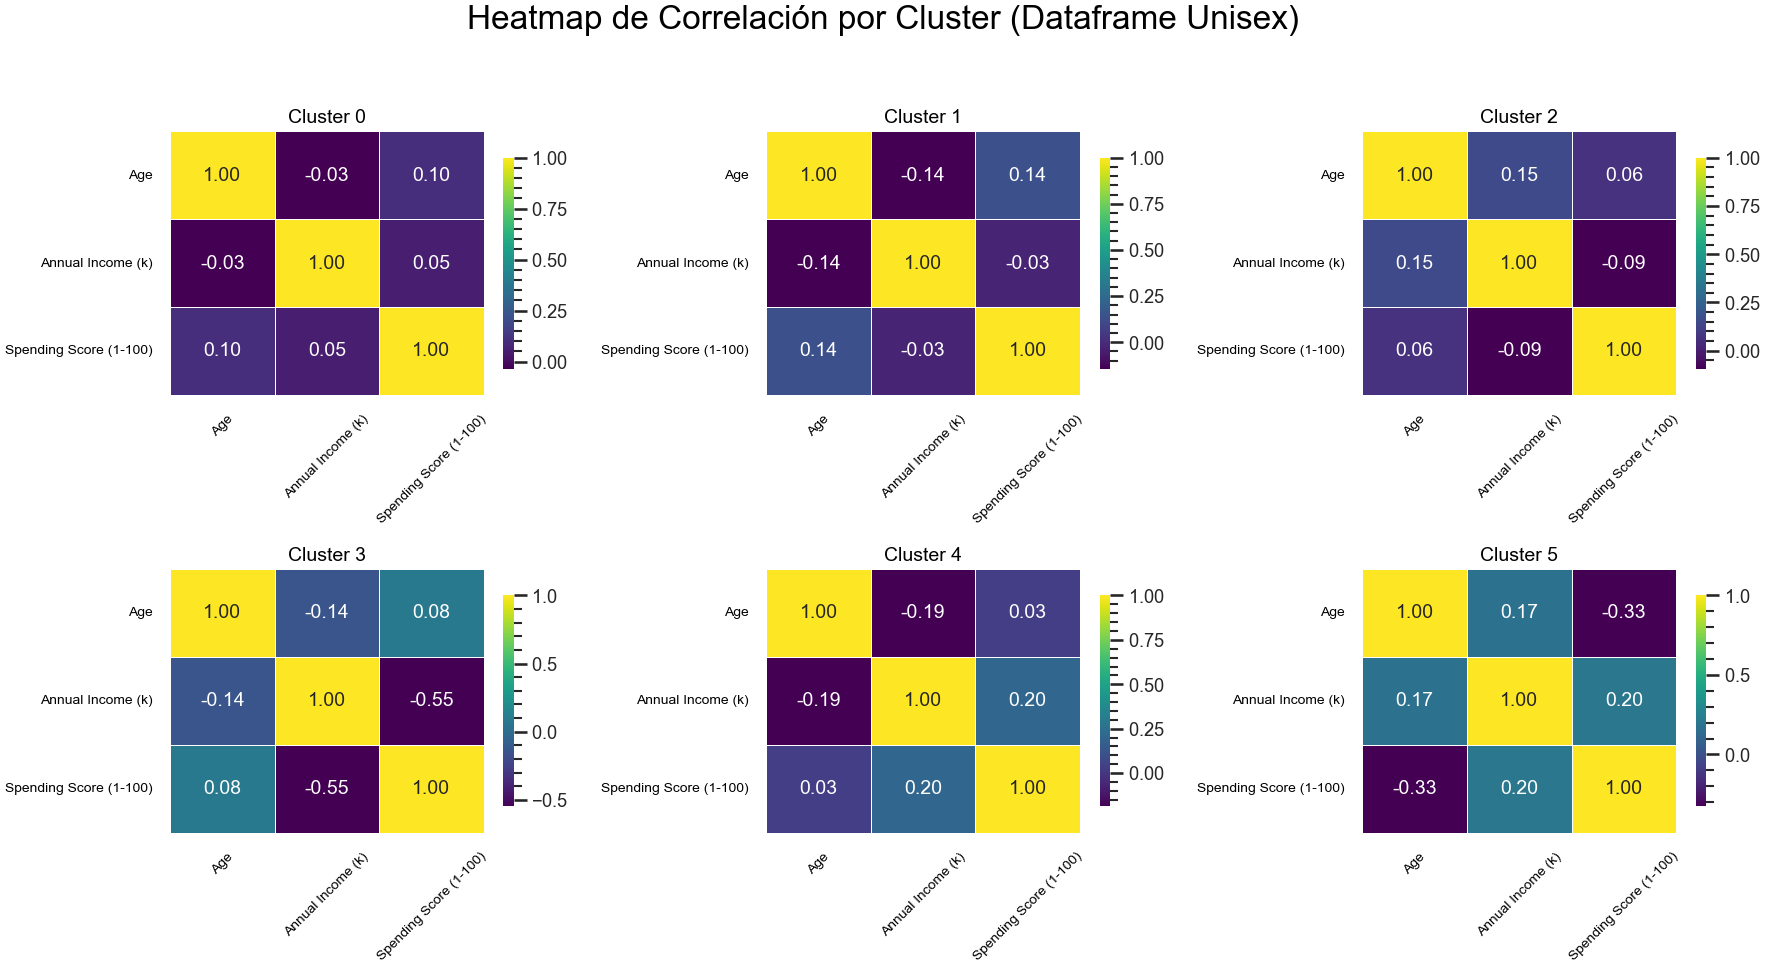
\includegraphics[width=0.8\textwidth]{plots_investing/Grafico 10.png}
    \caption{Heatmap of correlations between variables for each cluster.}
    \label{fig:miGrafico10}
\end{figure}

The heatmap analysis reveals two particularly relevant negative correlations, located in clusters 3 and 5:
\begin{enumerate}
    \item Cluster 3 shows a negative correlation of -0.55 between “Spending Score” and “Annual Income”, indicating that within this group, individuals with incomes between \$49,000 and \$69,000 and ages between 18 and 32 tend to exhibit purchasing behavior that is inversely proportional to their age.
    \item Cluster 5 exhibits a negative correlation of -0.33 between “Spending Score” and “Age”, suggesting that individuals aged between 45 and 57 with incomes between \$19,000 and \$33,000 tend to decrease their purchasing behavior as they age.
\end{enumerate}

Our initial conclusion was that our target audience was between 18 and 45 years old, combining both ranges with a spending score greater than 50. However, the income range required for these individuals to be considered high-potential customers was never specified. Thanks to the observed correlations (see Table~\ref{tab:spending_income}), it is now possible to evidence the significant influence of \emph{Annual Income} in this context.

The new hypothesis establishes that such individuals must have an income below \$49,000 or above \$69,000. To reach this conclusion, it will be necessary to verify it by exploring those individuals who register higher levels of spending relative to their incomes (see Table~\ref{tab:spending_income}).

We can conclude, therefore, that the hypothesis — according to which individuals earning less than \$49,000 or more than \$69,000, and who are between 18 and 45 years old, are more likely to be potential customers — is valid. Thus, the overall profile of a potential customer is defined as individuals between 18 and 45 years old who earn an annual income below \$49,000 or above \$69,000.

It should be noted that this profile will only be useful in cases where the individual's gender is unknown, but information on age and annual income is available.

\begin{table}[h]
    \centering
    \begin{tabular}{lc}
        \toprule
        \textbf{Income Range} & \textbf{Average Spending} \\
        \midrule
        0--49 & 58.96 \\
        50--68 & 49.25 \\
        69+   & 57.67 \\
        \bottomrule
    \end{tabular}
    \caption{Simple average spending by income group (ages 18--32)}
    \label{tab:spending_income}
\end{table}

\subsubsection{Dataset Division by Gender: Rationale and Justification}

Dividing the dataset into two subgroups—one for male customers and one for female customers—is based on the need to capture the particularities and nuances that each segment presents in terms of behavior and consumption characteristics. The following provides a detailed and well-founded explanation for this segmentation:


\begin{enumerate}
    \item \textbf{Differences in Behavior and Preferences:} Previous studies and empirical evidence indicate that, in many consumption contexts, men and women may exhibit different spending patterns and decision-making processes. By separating the dataset, the analysis of specific variables (such as \textit{Spending Score} and \textit{Annual Income}) is facilitated, allowing for the identification of correlations and trends particular to each gender. This enriches the analysis and enables the development of more tailored and personalized marketing and segmentation strategies.
    
    \item \textbf{Improved Profiling Accuracy:} The inherent heterogeneity in consumption behaviors is reinforced by the diversity of socioeconomic and cultural factors that influence each gender differently. By analyzing men and women separately, a more accurate profiling of potential customers is achieved, leading to the identification of segments with a high probability of conversion and the optimization of resources by focusing strategies on the specific characteristics of each subgroup.
    
    \item \textbf{Methodological and Academic Considerations:} From a methodological standpoint, dividing the dataset helps reduce internal variability and potential confounding effects that arise when mixing heterogeneous groups. This practice is consistent with the application of advanced clustering techniques, such as K-means, as a homogeneous analysis within each subgroup ensures that the validation indices and the cohesion and separation metrics are more representative of each gender's behavior. Moreover, this segmentation supports the applicability of winsorization methods and more robust statistical analysis, strengthening the interpretability of the results obtained.
    
    \item \textbf{Impact on Strategic Decision-Making:} Identifying specific patterns in each gender facilitates the development of targeted marketing strategies. For instance, by observing that certain age ranges or income levels are associated differently with spending in each segment, personalized campaigns can be designed to maximize customer acquisition and retention. This segmented approach is crucial in a competitive environment, where the adaptation and personalization of strategies become key differentiators for commercial success.
\end{enumerate}

In summary, dividing the dataset addresses a dual need: to improve the quality and accuracy of the analysis by reducing heterogeneity, and to provide a solid basis for generating potential customer profiles that accurately reflect the behavioral differences between men and women. This approach not only enhances the academic rigor of the study but also offers a practical tool for implementing effective and personalized marketing strategies.



\subsubsection{Profiling of Male Customers}

After segmenting the dataset, we proceed with the analysis of the subset corresponding to male customers, which is composed of 86 records. Although this number does not represent half of the total, it is sufficient to conduct a robust and meaningful study.

In the first instance, the correlations between the variables are examined to identify possible collinearities and relationships of interest, as illustrated in Figure~\ref{fig:miGrafico11}.

\begin{figure}[h]
    \centering
    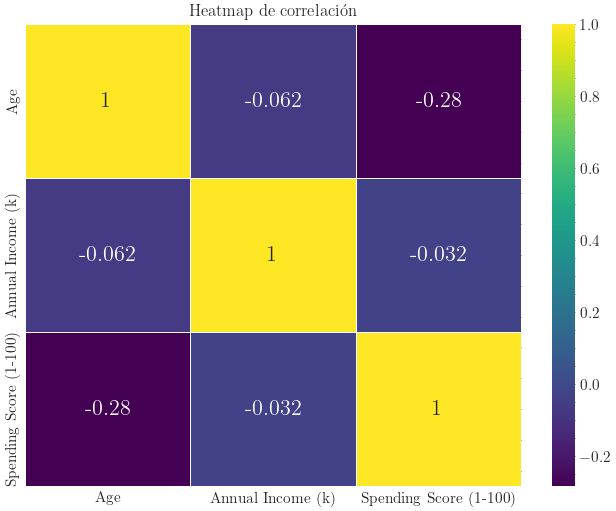
\includegraphics[width=0.4\textwidth]{plots_investing/Grafico 11.png}
    \caption{Heatmap of correlations between variables (male customers).}
    \label{fig:miGrafico11}
\end{figure}

Although a correlation of -0.28 was observed between the \textit{Spending Score (1-100)} variable and other variables, this value is not considered significant since it does not reach the threshold for a moderate correlation.

Next, the k-means method is applied to uncover underlying patterns in the data. Initially, the optimal number of clusters is determined using various statistical indices, the results of which are summarized in Table~\ref{tab:clusters_optimos_masculine}.

In Figure~\ref{fig:miGrafico12} these indices are shown, highlighting the delimited area and the positions of the optimal clusters according to each criterion.


\begin{table}[h]
    \centering
    \caption{Optimal Clusters by Metric (range [4,15])}
    \label{tab:clusters_optimos_masculine}
    \renewcommand{\arraystretch}{1.2}
    \begin{tabular}{@{}lccc@{}}
        \toprule
        \textbf{Metric}         & \textbf{Optimal Cluster 1} & \textbf{Optimal Cluster 2} & \textbf{Optimal Cluster 3} \\
        \midrule
        Silhouette Coefficient  & 5                        & 9                        & 11                       \\
        Dunn Index              & 4                        & 5                        & 11                       \\
        Calinski-Harabasz       & 10                       & 11                       & 12                       \\
        Davies-Bouldin          & 8                        & 11                       & 14                       \\
        \bottomrule
    \end{tabular}
\end{table}

\begin{figure}[h]
    \centering
    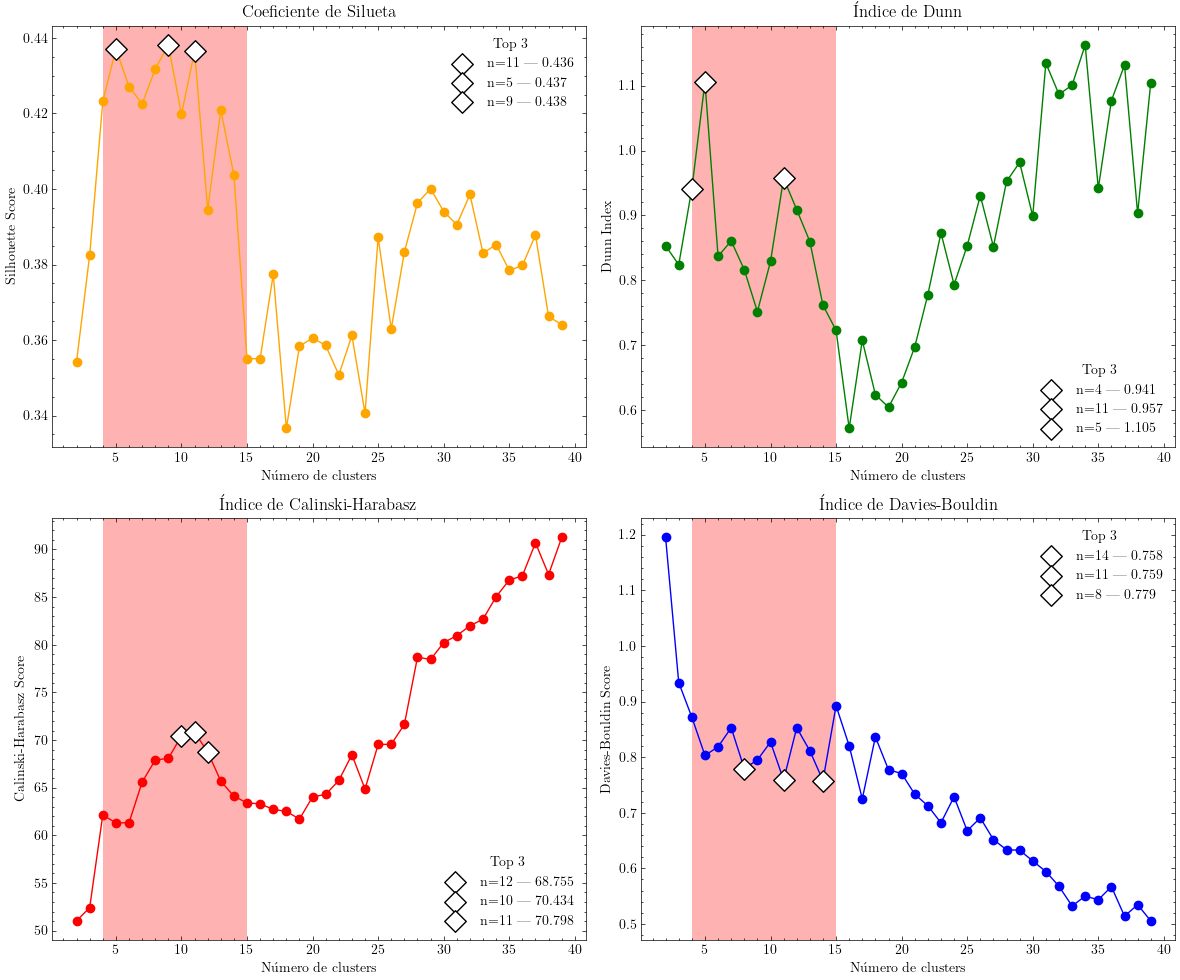
\includegraphics[width=0.8\textwidth]{plots_investing/Grafico 12.png}
    \caption{Indices for determining the optimal number of clusters.}
    \label{fig:miGrafico12}
\end{figure}

According to the various indices, it was determined that the optimal number of clusters is 11. With this parameter, the k-means model was trained and descriptive statistics were extracted for each group, as detailed in Table~\ref{tab:estadisticas_clusters_hombres_table}.


\begin{table}[h]
    \centering
    \resizebox{\textwidth}{!}{%
        \begin{tabular}{ccccccccccccc}
        \toprule
        Cluster & \multicolumn{3}{c}{Age} & \multicolumn{3}{c}{Annual Income (k\$)} & \multicolumn{3}{c}{Spend Score} & \multicolumn{3}{c}{Skew} \\
        \cmidrule(lr){2-4} \cmidrule(lr){5-7} \cmidrule(lr){8-10} \cmidrule(lr){11-13}
                & Mean   & Std   & Median  & Mean   & Std   & Median  & Mean   & Std   & Median  & Age    & Annual Income  & Spend Score \\
        \midrule
        \textbf{0}  & \textbf{52.78} & \textbf{4.74}  & \textbf{53.00} & \textbf{55.22} & \textbf{7.08}  & \textbf{54.00} & \textbf{49.22} & \textbf{5.63}  & \textbf{47.00} & \textbf{0.27}       & \textbf{-0.69}        & \textbf{0.97} \\
        \textbf{1}  & \textbf{35.17} & \textbf{4.00}  & \textbf{35.50} & \textbf{78.50} & \textbf{9.57}  & \textbf{76.00} & \textbf{88.00} & \textbf{8.70}  & \textbf{90.50} & \textbf{-0.45}      & \textbf{1.24} & \textbf{-0.95} \\
        \textbf{2}  & \textbf{39.78} & \textbf{5.09}  & \textbf{40.00} & \textbf{86.22} & \textbf{12.71} & \textbf{86.00} & \textbf{10.44} & \textbf{6.60}  & \textbf{10.00} & \textbf{0.10}       & \textbf{1.23} & \textbf{-0.24} \\
        \textbf{3}  & \textbf{21.60} & \textbf{3.69}  & \textbf{19.50} & \textbf{56.90} & \textbf{7.42}  & \textbf{59.50} & \textbf{52.60} & \textbf{5.76}  & \textbf{54.50} & \textbf{0.53}       & \textbf{-0.37}        & \textbf{-0.95} \\
        \textbf{4}  & \textbf{24.40} & \textbf{5.62}  & \textbf{23.00} & \textbf{24.70} & \textbf{7.39}  & \textbf{24.50} & \textbf{73.80} & \textbf{15.80} & \textbf{76.00} & \textbf{0.80} & \textbf{0.35}         & \textbf{-1.11} \\
        5           & 40.57        & 5.74         & 40.00         & 46.71        & 14.76         & 43.00         & 44.29        & 10.23         & 41.00         & 0.08         & 0.20         & 0.65 \\
        \textbf{6}  & \textbf{55.50} & \textbf{10.82} & \textbf{56.50} & \textbf{24.00} & \textbf{6.07}  & \textbf{21.50} & \textbf{11.17} & \textbf{9.99}  & \textbf{8.50}  & \textbf{-0.99} & \textbf{0.85}  & \textbf{1.33} \\
        \textbf{7}  & \textbf{29.40} & \textbf{2.41}  & \textbf{28.00} & \textbf{97.80} & \textbf{16.84} & \textbf{88.00} & \textbf{69.80} & \textbf{4.87}  & \textbf{69.00} & \textbf{0.47}       & \textbf{1.66}  & \textbf{-0.38} \\
        \textbf{8}  & \textbf{20.75} & \textbf{2.87}  & \textbf{19.50} & \textbf{76.25} & \textbf{3.59}  & \textbf{75.50} & \textbf{8.00}  & \textbf{3.56}  & \textbf{7.50}  & \textbf{1.85} & \textbf{0.89}  & \textbf{0.27} \\
        \textbf{9}  & \textbf{54.80} & \textbf{5.36}  & \textbf{58.00} & \textbf{82.80} & \textbf{8.79}  & \textbf{85.00} & \textbf{20.40} & \textbf{10.41} & \textbf{15.00} & \textbf{-0.66}      & \textbf{-0.38}        & \textbf{1.01} \\
        10          & 67.22        & 2.33         & 67.00         & 54.67        & 8.12          & 54.00         & 50.11        & 6.09          & 51.00         & -0.50        & -0.06        & -0.12 \\
        \bottomrule
        \end{tabular}%
    }
    \caption{Statistics by cluster (male clients). Rows where any skew value exceeds 0.7 or is below -0.7 are highlighted in bold.}
    \label{tab:estadisticas_clusters_hombres_table}
\end{table}


\begin{table}[p]
    \caption{Variables and parameters used for outlier elimination (Clusters 0, 1, 2, 3, 4, 6, 7, 8, and 9)}
    \label{tab:outliers}
    \centering
    \begin{tabularx}{\textwidth}{c c c c c X}
    \toprule
    Index & Variable & Interval & Factor & Cluster & Description \\
    \midrule
    0  & Spending Score (1-100) & [0, 0.2]   & 1.5 & 0 & The top 20\% of extreme values was removed and outliers were detected using an IQR factor of 1.5. (Cluster 0) \\
    1  & Annual Income (k)      & [0, 0.2]   & 1   & 1 & The top 20\% of extreme values was removed and outliers were detected using an IQR factor of 1. (Cluster 1) \\
    2  & Spending Score (1-100) & [0.3, 0]   & 1   & 1 & The bottom 30\% of extreme values was removed and outliers were detected using an IQR factor of 1. (Cluster 1) \\
    3  & Annual Income (k)      & [0, 0.2]   & 1.5 & 2 & The top 20\% of extreme values was removed and outliers were detected using an IQR factor of 1.5. (Cluster 2) \\
    4  & Spending Score (1-100) & [0.1, 0]   & 1   & 3 & The bottom 10\% of extreme values was removed and outliers were detected using an IQR factor of 1. (Cluster 3) \\
    5  & Spending Score (1-100) & [0.1, 0]   & 1.5 & 4 & The bottom 10\% of extreme values was removed and outliers were detected using an IQR factor of 1.5. (Cluster 4) \\
    6  & Age                    & [0, 0.1]   & 1.5 & 4 & The top 10\% of extreme values was removed and outliers were detected using an IQR factor of 1.5. (Cluster 4) \\
    7  & Age                    & [0.2, 0]   & 1   & 6 & The bottom 20\% of extreme values was removed and outliers were detected using an IQR factor of 1. (Cluster 6) \\
    8  & Spending Score (1-100) & [0, 0.2]   & 1.5 & 6 & The top 20\% of extreme values was removed and outliers were detected using an IQR factor of 1.5. (Cluster 6) \\
    9  & Annual Income (k)      & [0, 0.2]   & 0.5 & 6 & The top 20\% of extreme values was removed and outliers were detected using an IQR factor of 0.5. (Cluster 6) \\
    10 & Annual Income (k)      & [0, 0.2]   & 1.5 & 7 & The top 20\% of extreme values was removed and outliers were detected using an IQR factor of 1.5. (Cluster 7) \\
    11 & Age                    & [0, 0.3]   & 1   & 8 & The top 30\% of extreme values was removed and outliers were detected using an IQR factor of 1. (Cluster 8) \\
    12 & Annual Income (k)      & [0, 0.3]   & 0.5 & 8 & The top 30\% of extreme values was removed and outliers were detected using an IQR factor of 0.5. (Cluster 8) \\
    13 & Spending Score (1-100) & [0, 0.2]   & 0.5 & 9 & The top 20\% of extreme values was removed and outliers were detected using an IQR factor of 0.5. (Cluster 9) \\
    \bottomrule
    \end{tabularx}
\end{table}

Table~\ref{tab:outliers} meticulously details the modifications made and the IQR factors used to detect outliers in each cluster. Subsequently, Table~\ref{tab:estadisticas_winsorizadas} presents the data after winsorization.


\begin{table}[h]
    \centering
    \resizebox{\textwidth}{!}{%
    \begin{tabular}{ccccccccccccc}
        \toprule
        Cluster & \multicolumn{3}{c}{Age} & \multicolumn{3}{c}{Annual Income (k\$)} & \multicolumn{3}{c}{Spend Score} & \multicolumn{3}{c}{Skew} \\
        \cmidrule(lr){2-4} \cmidrule(lr){5-7} \cmidrule(lr){8-10} \cmidrule(lr){11-13}
                & Mean   & Std   & Median  & Mean   & Std   & Median  & Mean   & Std   & Median  & Age    & Annual Income  & Spend Score \\
        \midrule
        0  & 52.78 & 4.74  & 53.00 & 55.22 & 7.08  & 54.00 & 48.78 & 4.76  & 47.00 & 0.27  & -0.69 & 0.57 \\
        1  & 35.17 & 4.00  & 35.50 & 77.00 & 6.70  & 76.00 & 91.42 & 3.42  & 90.50 & -0.45 & 0.64  & 0.63 \\
        2  & 39.78 & 5.09  & 40.00 & 84.56 & 9.28  & 86.00 & 10.44 & 6.60  & 10.00 & 0.10  & 0.31  & -0.24 \\
        3  & 21.60 & 3.69  & 19.50 & 56.90 & 7.42  & 59.50 & 53.10 & 4.77  & 54.50 & 0.53  & -0.37 & -0.43 \\
        4  & 24.00 & 4.88  & 23.00 & 24.70 & 7.39  & 24.50 & 76.00 & 11.30 & 76.00 & 0.45  & 0.35  & 0.07 \\
        5  & 40.57 & 5.74  & 40.00 & 46.71 & 14.76 & 43.00 & 44.29 & 10.23 & 41.00 & 0.08  & 0.20  & 0.65 \\
        6  & 58.00 & 6.60  & 56.50 & 23.50 & 5.24  & 21.50 & 8.67  & 5.50  & 8.50  & 0.41  & 0.67  & -0.00 \\
        7  & 29.40 & 2.41  & 28.00 & 92.80 & 7.50  & 88.00 & 69.80 & 4.87  & 69.00 & 0.47  & 0.60  & -0.38 \\
        8  & 19.50 & 0.58  & 19.50 & 75.25 & 2.06  & 75.50 & 8.00  & 3.56  & 7.50  & 0.00  & -0.20 & 0.27 \\
        9  & 54.80 & 5.36  & 58.00 & 82.80 & 8.79  & 85.00 & 18.40 & 7.09  & 15.00 & -0.66 & -0.38 & 0.41 \\
        10 & 67.22 & 2.33  & 67.00 & 54.67 & 8.12  & 54.00 & 50.11 & 6.09  & 51.00 & -0.50 & -0.06 & -0.12 \\
        \bottomrule
    \end{tabular}%
    }
    \caption{Cluster statistics (male clients) after winsorization.}
    \label{tab:estadisticas_winsorizadas}
\end{table}

Knowing the distribution of the data, the correlations between the variables within each cluster are examined below to further explore the classification conditions, as illustrated in Figure~\ref{fig:miGrafico14}.

\begin{figure}[p]
    \centering
    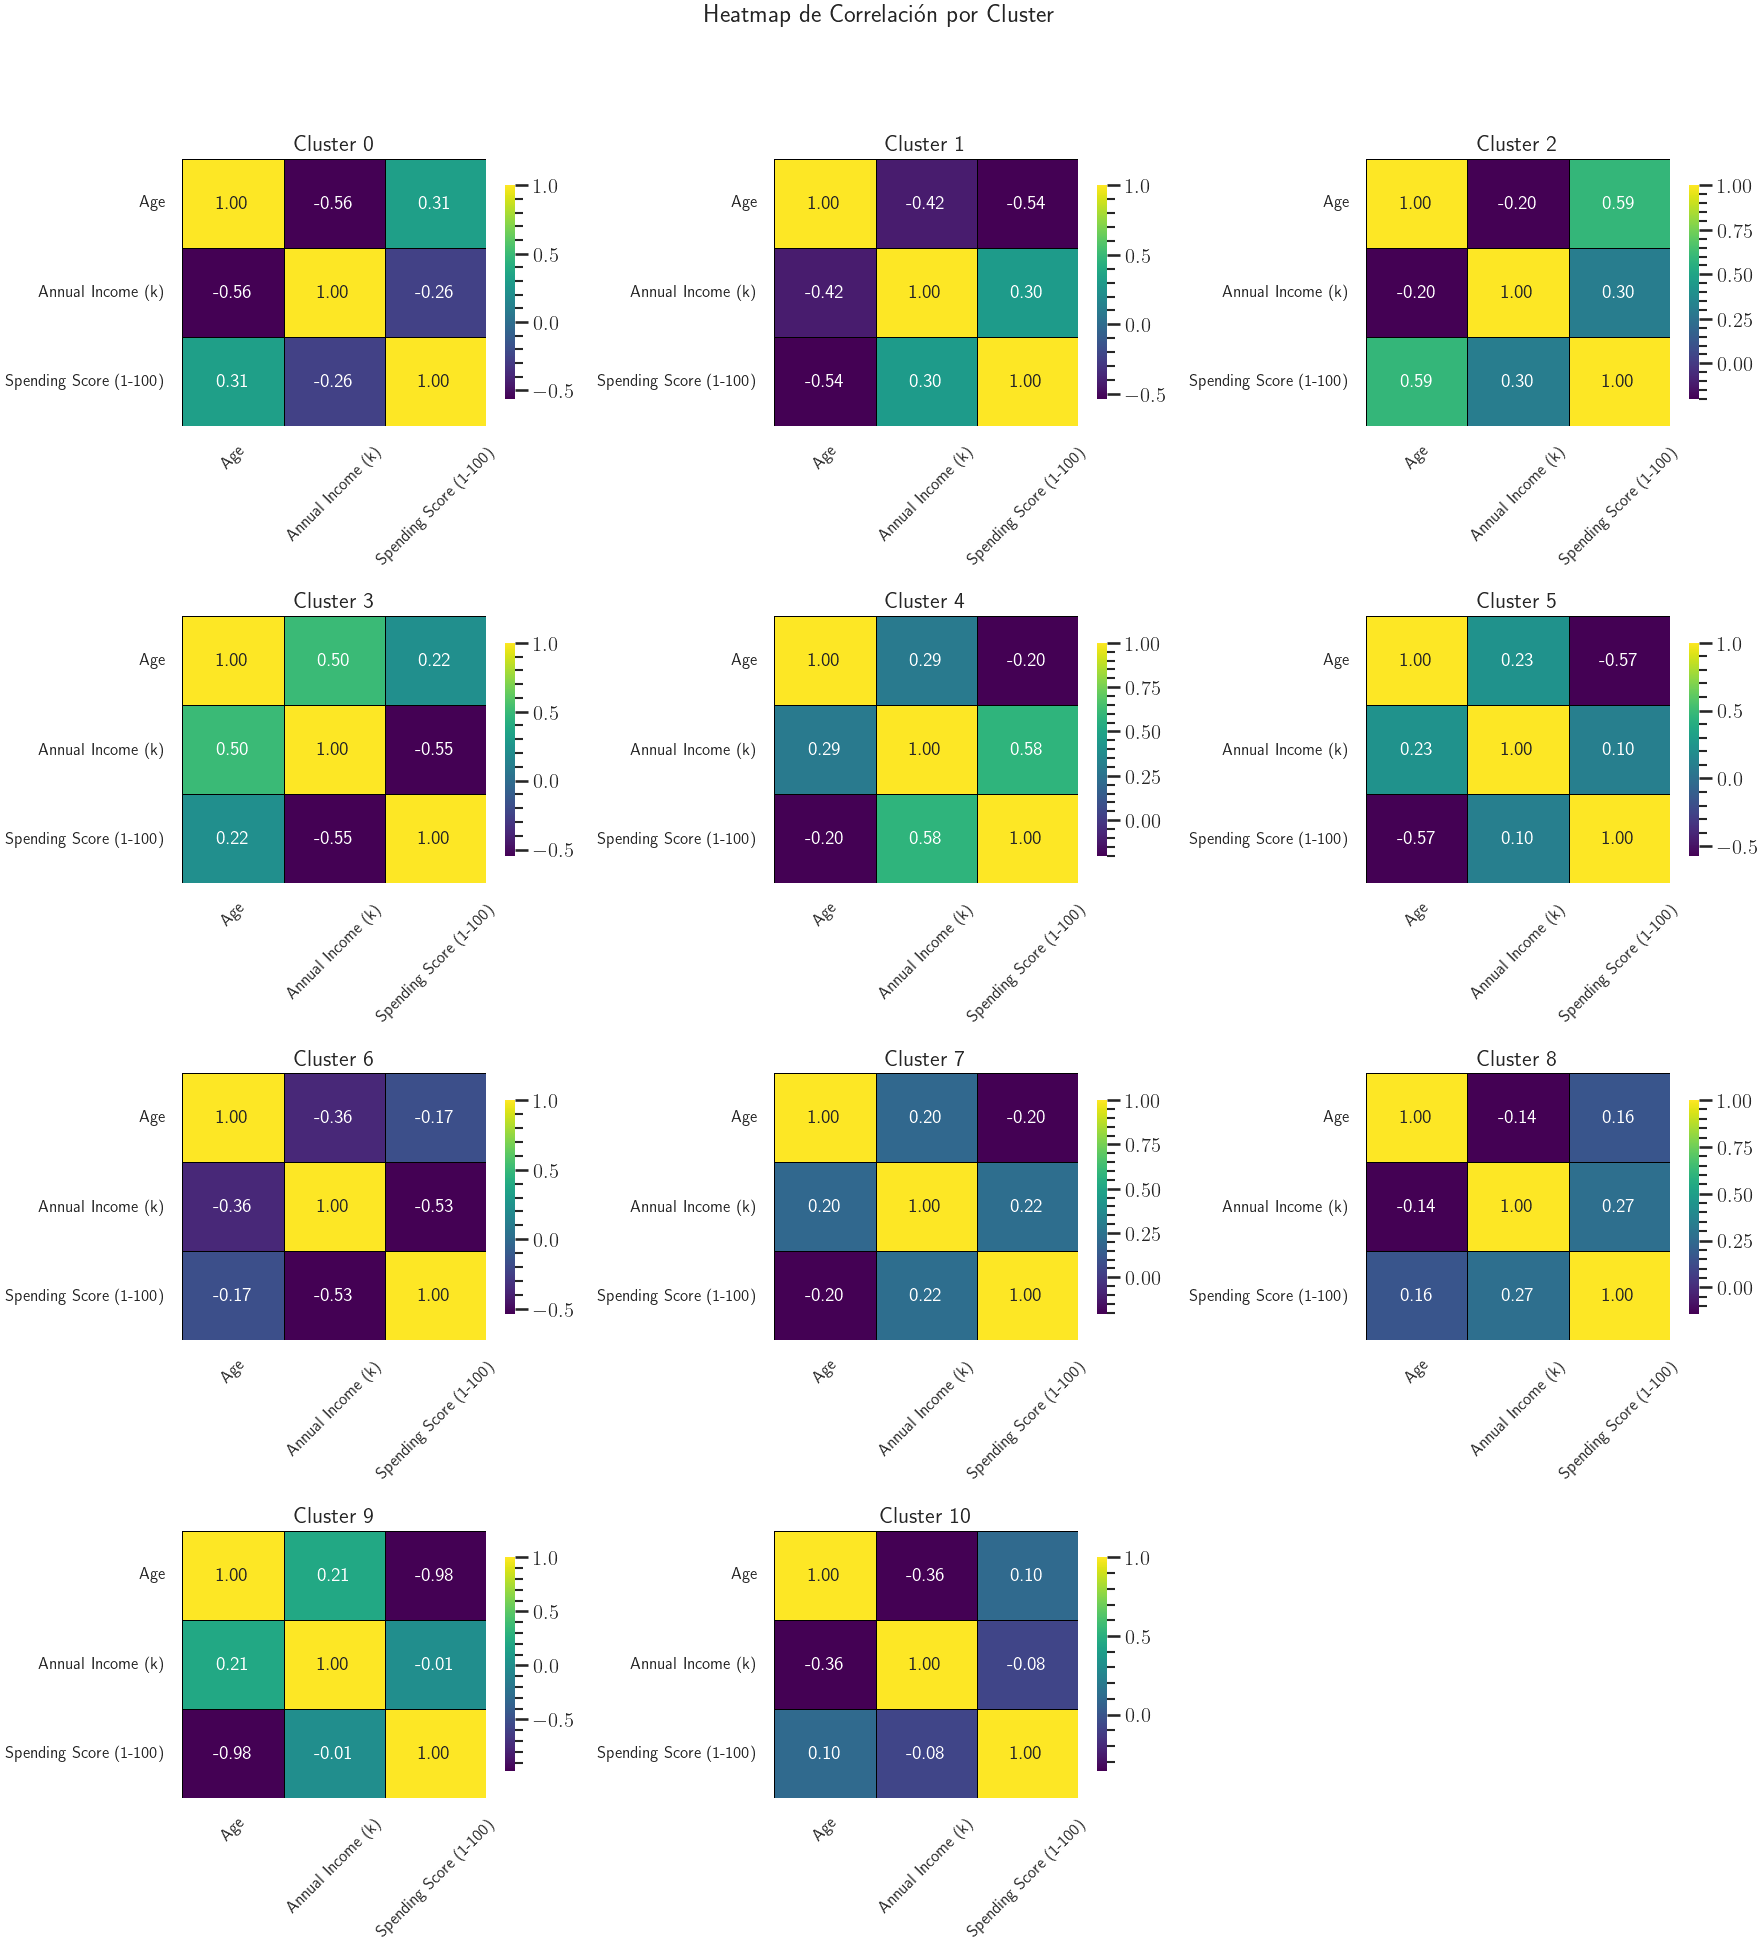
\includegraphics[width=0.8\textwidth]{plots_investing/Grafico 14.png}
    \caption{Heat map of correlations between variables for each cluster.}
    \label{fig:miGrafico14}
\end{figure}

Based on the correlations shown in Figure~\ref{fig:miGrafico14} and the descriptive statistics, it is possible to draw conclusions of special interest:


\paragraph{Clusters with high income and high spending:}
\begin{itemize}
    \item \textbf{Cluster 1} (31.2--39.2 years): It exhibits high incomes (70.3--83.7) and very high spending (88.0--94.8).
    \item \textbf{Cluster 7} (27.0--31.8 years): It records even higher incomes (85.3--100.3) and moderately high spending (64.9--74.7).
\end{itemize}
These groups represent consumers with high purchasing power and intense consumption patterns.

\paragraph{Clusters with low income and low spending:}
\begin{itemize}
    \item \textbf{Cluster 6} (51.4--64.6 years): It is characterized by reduced incomes (17.9--30.1) and limited spending (3.2--14.2).
    \item \textbf{Cluster 2} (34.7--44.9 years): Although its incomes are high (75.3--93.8), the spending is extremely low (3.8--17.0).
\end{itemize}
While Cluster 6 might represent people nearing retirement with certain economic limitations, Cluster 2 suggests consumers with a high capacity to save and a low propensity to spend.

\paragraph{Clusters with low income but high spending:}
\begin{itemize}
    \item \textbf{Cluster 4} (18.8--30.0 years): With limited incomes (17.3--32.1) and high spending (64.7--87.3), this group probably represents young people with less financial stability, but with a marked tendency to consume.
\end{itemize}

\paragraph{Clusters of older ages with controlled spending:}
\begin{itemize}
    \item \textbf{Cluster 9} (49.4--60.2 years): Although it presents high incomes (74.0--91.6), spending remains at low to moderate levels (10.0--30.8).
    \item \textbf{Cluster 10} (64.9--69.6 years): It is characterized by having both income and spending at moderate levels.
\end{itemize}
These groups are associated with mature individuals exhibiting more conservative financial behaviors.

\paragraph{Notable correlations:}
\begin{itemize}
    \item \textbf{Positive (green):} These are observed in Cluster 2 (age and income are positively correlated, despite low spending) and in Clusters 3 and 4 (young people with high spending).
    \item \textbf{Negative (red):} These are evident in Clusters 6 and 9, suggesting that in older ages there tends to be lower spending.
    \item \textbf{Auto-correlation (orange):} This is noticeable in Clusters 1 and 3, indicating consistent internal patterns within these segments.
\end{itemize}

\paragraph{Segments of greatest commercial interest:}

\textbf{Cluster 1} (31.2--39.2 years):
\begin{itemize}
    \item High incomes: 70.3--83.7.
    \item Very high spending: 88.0--94.8.
    \item Positive correlation between income and spending.
\end{itemize}
This segment is especially attractive due to its high purchasing power and marked propensity to consume. It likely comprises young adults with financial stability and a strong desire to acquire goods and services.

\textbf{Cluster 4} (18.8--30.0 years):
\begin{itemize}
    \item Low incomes: 17.3--32.1.
    \item High spending: 64.7--87.3.
    \item A positive correlation in spending and a negative correlation in income are observed.
\end{itemize}
Despite their limited incomes, this group shows a notable inclination to consume, which could indicate the presence of students or young professionals willing to prioritize spending over saving. Thus, it constitutes a potential market for aspirational or affordable luxury products.

\textbf{Cluster 3} (17.9--25.3 years):
\begin{itemize}
    \item Medium incomes: 49.5--64.3.
    \item Medium-high spending: 48.3--57.9.
    \item High correlation between income and spending.
\end{itemize}
This segment probably groups young individuals with stable employment, inclined to invest in technology, fashion, or entertainment. With incomes higher than those in Cluster 4, their dependency on credit is potentially lower.



\subsubsection{Profiling of Female Customers}

After profiling the potential customers, a specific analysis of the female gender is carried out, in which the passion for science and reason merges with the art of understanding human behaviors. The method employed is analogous to that used for the male gender; however, a particular phenomenon has been identified: the correlation between the \textit{spending score} and age reaches approximately \(-0.4\) (see Figure~\ref{fig:miGrafico15}). This finding, which contrasts with both the analysis of the male gender and the overall heatmap, suggests that as age increases, women tend to show less interest in products. Far from being a mere number, this result invites further analysis by incorporating new variables and using techniques such as \textit{k-means}, in a sincere homage to science and the power of reasoning.

\begin{figure}[h]
    \centering
    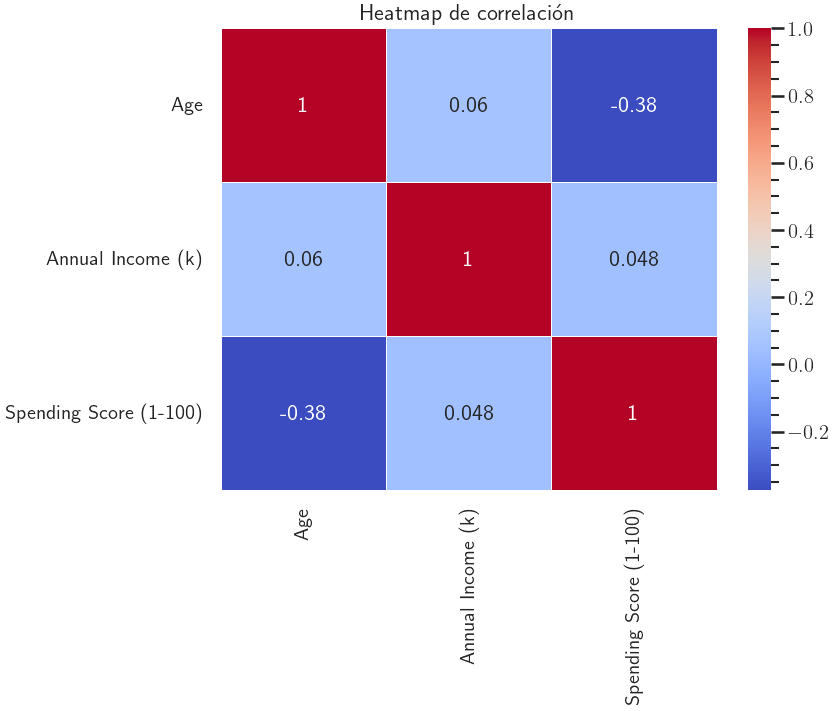
\includegraphics[width=0.8\textwidth]{plots_investing/Grafico 15.png}
    \caption{Heat map of correlations between variables for each cluster.}
    \label{fig:miGrafico15}
\end{figure}

The determination of the optimal number of clusters was carried out based on various indicators (see Figure~\ref{fig:miGrafico16}). The convergence of these indicators suggests the formation of 6 clusters, which contrasts with the segmentation observed in the male gender. This lower diversity in the female dataset implies a greater concentration of information in each group, thereby strengthening the robustness and accuracy of the applied classification rules.

\begin{figure}[h]
    \centering
    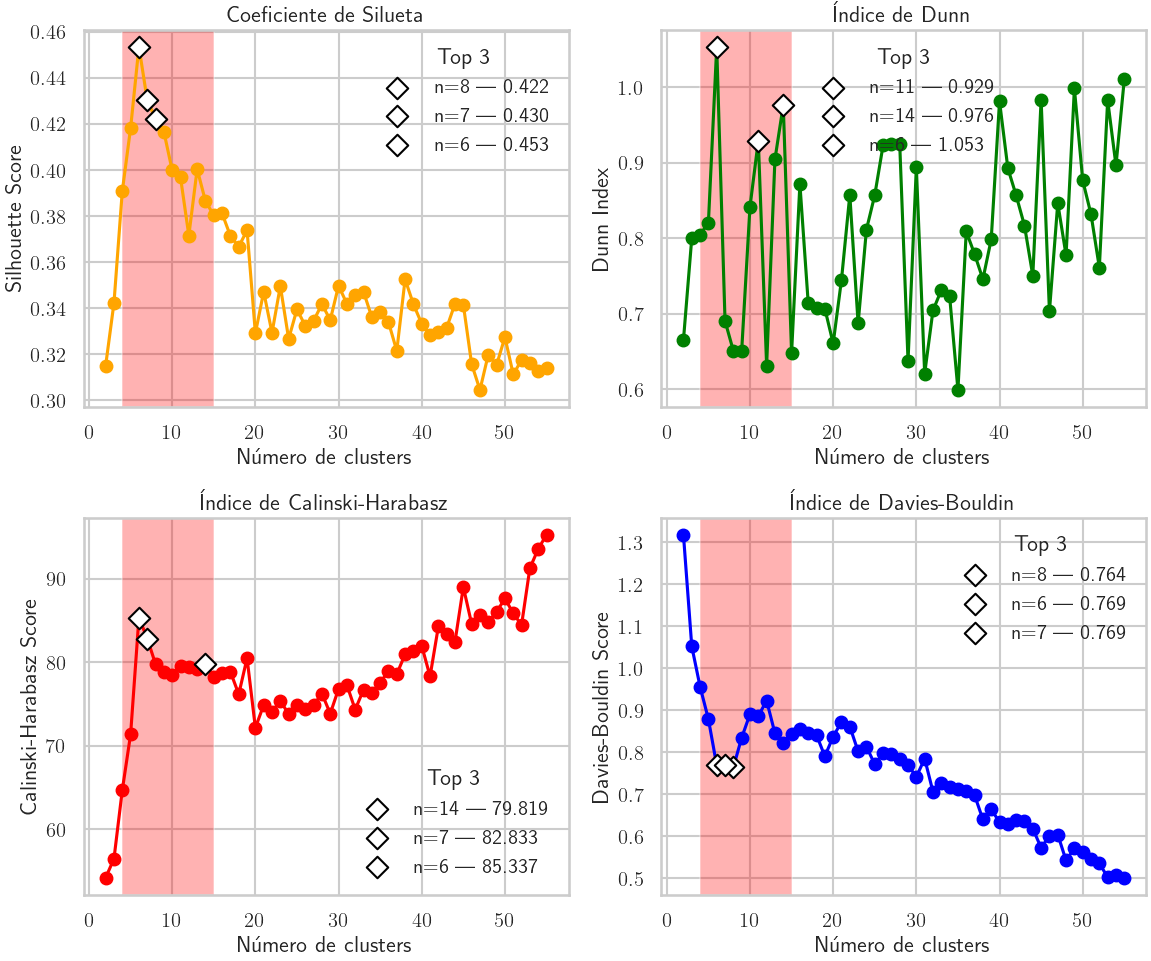
\includegraphics[width=0.8\textwidth]{plots_investing/Grafico 16.png}
    \caption{Heat map of correlations between variables for each cluster.}
    \label{fig:miGrafico16}
\end{figure}

Table~\ref{tab:clusters_optimos} summarizes the optimal points selected according to each metric used:

\begin{table}[htbp]
    \centering
    \caption{\textbf{Optimal Clusters by Metric}}
    \label{tab:clusters_optimos}
    \renewcommand{\arraystretch}{1.2}
    \begin{tabular}{@{}lccc@{}}
        \toprule
        \textbf{Metric}         & \textbf{Optimal Cluster 1} & \textbf{Optimal Cluster 2} & \textbf{Optimal Cluster 3} \\
        \midrule
        Silhouette Coefficient   & 6                       & 7                        & 10                      \\
        Dunn Index               & 4                       & 5                        & 6                       \\
        Calinski-Harabasz        & 6                       & 9                        & 11                      \\
        Davies-Bouldin           & 6                       & 7                        & 9                       \\
        \bottomrule
    \end{tabular}
\end{table}

With the \textit{k-means} algorithms trained for the optimal number of clusters, the classification condition statistics were examined (see Table~\ref{tab:estadisticas_femenine}). As expected, clusters with skewed distributions were identified, with the results corresponding to Clusters 2 and 3 highlighted in bold. To improve the symmetry of the groups, the winsorization technique was applied, whose results are shown in Table~\ref{tab:estadisticas_femenine_winsorización}.

\begin{table}[b]
    \centering
    \resizebox{\textwidth}{!}{%
    \begin{tabular}{ccccccccccccc}
        \toprule
        Cluster & \multicolumn{3}{c}{Age} & \multicolumn{3}{c}{Annual Income (k\$)} & \multicolumn{3}{c}{Spend Score} & \multicolumn{3}{c}{Skew} \\
        \cmidrule(lr){2-4} \cmidrule(lr){5-7} \cmidrule(lr){8-10} \cmidrule(lr){11-13}
                & Mean   & Std   & Median  & Mean   & Std   & Median  & Mean   & Std   & Median  & Age    & Annual Income  & Spend Score \\
        \midrule
         0     & 54.08  & 7.97  & 50.00   & 53.24  & 8.76  & 54.00   & 49.52  & 6.19  & 50.00   & 0.67   & 0.04         & -0.27 \\
         \textbf{1}     & \textbf{44.60}  & \textbf{7.66}  & \textbf{44.00}   & \textbf{92.33}  & \textbf{16.44} & \textbf{88.00}   & \textbf{21.60}  & \textbf{9.70}  & \textbf{22.00}   & \textbf{0.20}   & \textbf{0.72}         & \textbf{0.04}  \\
         \textbf{2}     & \textbf{25.46}  & \textbf{5.22}  & \textbf{23.00}   & \textbf{25.69}  & \textbf{8.24}  & \textbf{23.00}   & \textbf{80.54}  & \textbf{10.70} & \textbf{77.00}   & \textbf{1.03}   & \textbf{0.36}         & \textbf{0.70}  \\
         \textbf{3}     & \textbf{32.19}  & \textbf{3.08}  & \textbf{32.00}   & \textbf{86.05}  & \textbf{14.16} & \textbf{79.00}   & \textbf{81.67}  & \textbf{7.83}  & \textbf{83.00}   & \textbf{0.52}   & \textbf{1.10}         & \textbf{-0.00} \\
         4     & 41.54  & 10.26 & 42.00   & 26.54  & 7.76  & 28.00   & 20.69  & 11.93 & 17.00   & -0.41  & 0.14         & 0.13 \\
         5     & 27.96  & 6.67  & 27.00   & 57.36  & 10.98 & 60.00   & 47.12  & 8.19  & 47.00   & 0.34   & -0.39        & -0.15 \\
        \bottomrule
    \end{tabular}%
    }
    \caption{Cluster Statistics (female customers)}
    \label{tab:estadisticas_femenine}
\end{table}

\begin{table}[b]
    \centering
    \resizebox{\textwidth}{!}{%
    \begin{tabular}{ccccccccccccc}
        \toprule
        Cluster & \multicolumn{3}{c}{Age} & \multicolumn{3}{c}{Annual Income (k\$)} & \multicolumn{3}{c}{Spend Score} & \multicolumn{3}{c}{Skew} \\
        \cmidrule(lr){2-4} \cmidrule(lr){5-7} \cmidrule(lr){8-10} \cmidrule(lr){11-13}
                & Mean   & Std   & Median  & Mean   & Std   & Median  & Mean   & Std   & Median  & Age    & Annual Income  & Spend Score \\
        \midrule
         0     & 54.08  & 7.97  & 50.00   & 53.24  & 8.76  & 54.00   & 49.52  & 6.19  & 50.00   & 0.63   & 0.04         & -0.25 \\
         1     & 44.60  & 7.66  & 44.00   & 92.33  & 16.44 & 88.00   & 21.60  & 9.70  & 22.00   & 0.18   & 0.65         & 0.04  \\
         2     & 24.69  & 3.86  & 23.00   & 25.69  & 8.24  & 23.00   & 80.54  & 10.70 & 77.00   & 0.54   & 0.32         & 0.62  \\
         3     & 32.19  & 3.08  & 32.00   & 84.76  & 11.55 & 79.00   & 81.67  & 7.83  & 83.00   & 0.48   & 0.59         & -0.00 \\
         4     & 41.54  & 10.26 & 42.00   & 26.54  & 7.76  & 28.00   & 20.69  & 11.93 & 17.00   & -0.36  & 0.12         & 0.11  \\
         5     & 27.96  & 6.67  & 27.00   & 57.36  & 10.98 & 60.00   & 47.12  & 8.19  & 47.00   & 0.32   & -0.37        & -0.14 \\
        \bottomrule
    \end{tabular}%
    }
    \caption{Cluster Statistics (female customers) after winsorization}
    \label{tab:estadisticas_femenine_winsorización}
\end{table}

The correlation analysis using the heatmap (Figure~\ref{fig:miGrafico17}) provides enriching conclusions about the behavior of the clusters based on age, annual income, and the \textit{spending score}. In particular:
\begin{figure}[h]
    \centering
    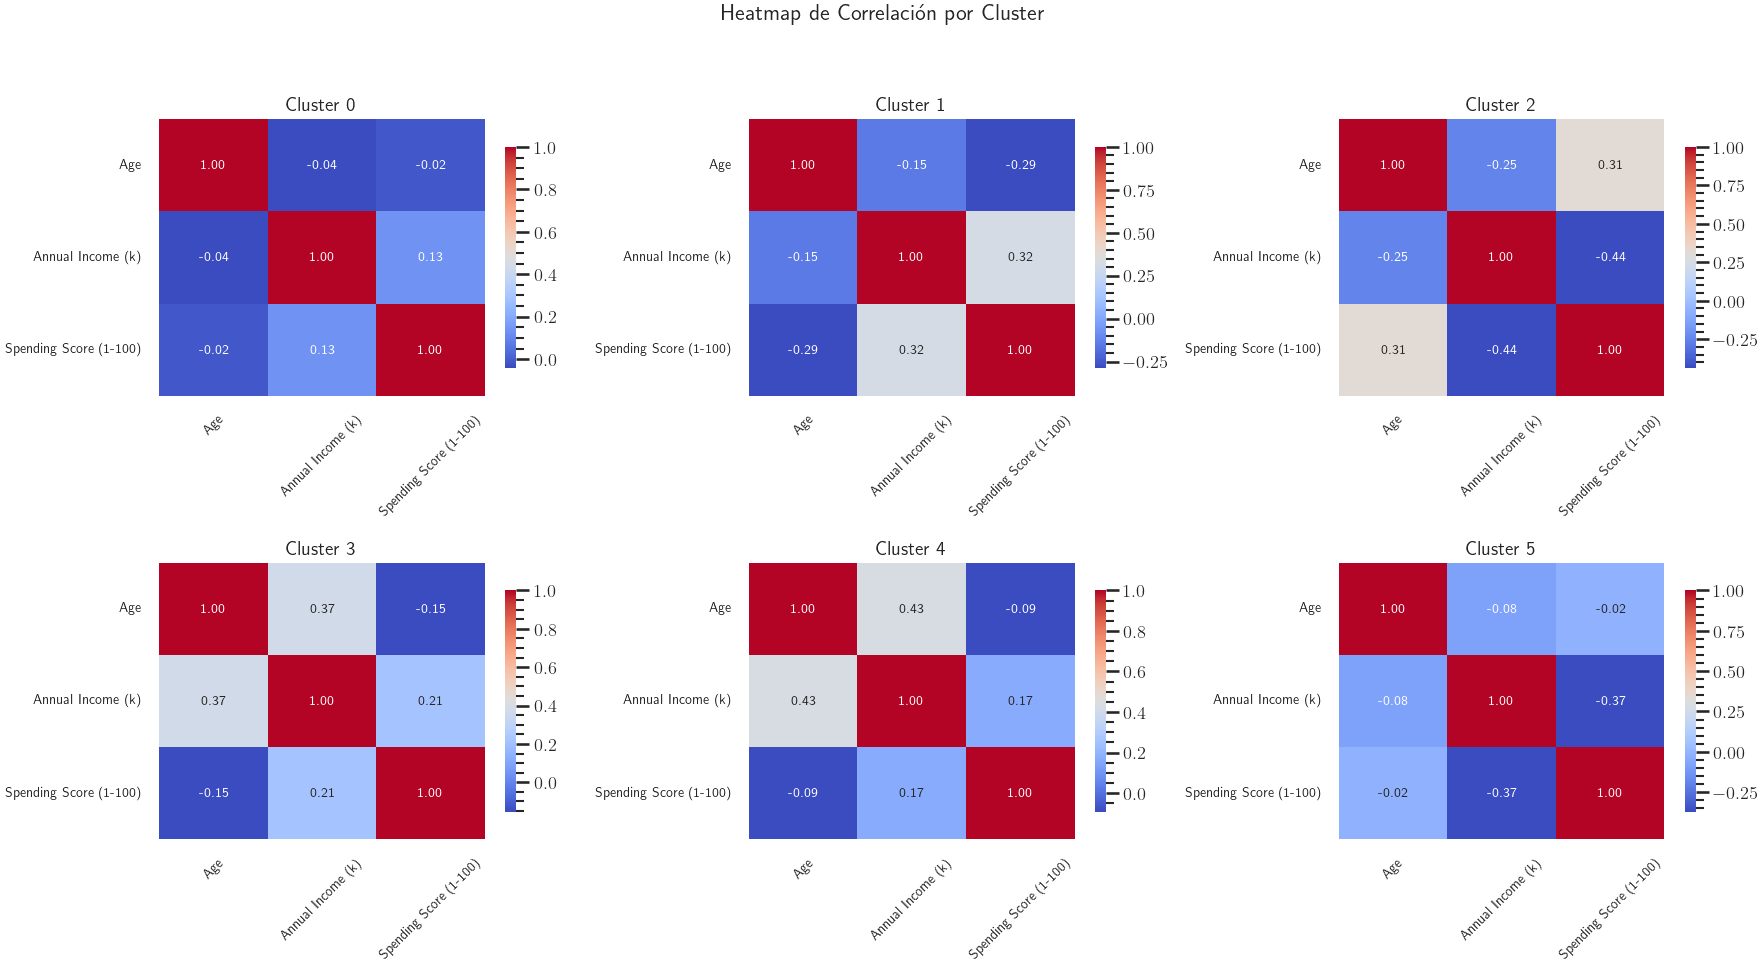
\includegraphics[width=0.8\textwidth]{plots_investing/Grafico 17.png}
    \caption{Heat map of correlations between variables for each cluster.}
    \label{fig:miGrafico17}
\end{figure}
\begin{itemize}
    \item \textbf{Differentiation of clusters by ranges:} Each cluster groups individuals who share specific ranges of age, income, and spending. For example, Cluster 2 brings together young women (20.8--28.6 years) with low annual incomes (17.5--33.9) and high spending (69.8--91.2), while Cluster 0 groups older women (46.1--62.1 years) with moderate incomes and spending.
    \item \textbf{Significant correlations:} In Cluster 2, a strong negative correlation (less than \(-0.4\)) between annual income and the \textit{spending score} is evident, suggesting that in this group, as income increases, spending tends to decrease. In contrast, Cluster 4 shows a significant positive correlation (greater than \(0.4\)) between age and annual income, indicating that in this group, age is associated with a slight increase in income. Clusters 0, 1, 3, and 5 do not present statistically relevant correlations among the analyzed variables.
    \item \textbf{Interpretation of correlations in orange:} The correlations highlighted in orange indicate that, within the same cluster, one variable maintains strong links with two different relationships. This phenomenon can be interpreted as a sign of consistency in the behavior of that variable, reflecting the underlying harmony in the analysis.
    \item \textbf{Practical applications:} These findings allow for the design of segmented marketing strategies. For example, in Cluster 2, campaigns could be developed targeted at young women with low incomes but a high propensity to spend, incentivizing consumption through offers or promotions. On the other hand, Cluster 4, with its positive association between age and income, could be the focus of strategies oriented towards experience and financial stability.
\end{itemize}

Finally, two groups of special interest for the commercial strategy are highlighted:


\begin{itemize}
    \item \textbf{Cluster 3 (29.1--35.3 years):} This segment exhibits high incomes (73.2--96.3) and a high \textit{spending score} (73.8--89.5), positioning it as an ideal candidate for premium products or services.
    \item \textbf{Cluster 2 (20.8--28.6 years):} Although its incomes are relatively low (17.5--33.9), this group shows notable spending behavior (69.8--91.2), evidencing a high propensity to consume. This makes it an attractive opportunity for promotional campaigns and affordable products, targeted at a young and dynamic audience.
\end{itemize}

In summary, the segmentation of the female gender not only differentiates customers according to ranges of age, income, and spending but also reveals significant relationships among these variables. This analysis, inspired by scientific rigor and a love for reason, paves the way for designing marketing strategies tailored to the particularities of each segment, merging technical precision with a deep sensitivity to human behavior.


\subsection{Applied Methods}

\lettrine[lines=3, loversize=0.01, lhang=0.01]{\scalebox{0.9}{\initfamily I}}{n} this section the applied methods are addressed, which constitute the backbone of the analysis. Techniques for clustering – with the K-means algorithm as the central axis – are combined with validation and optimization strategies, such as the elbow method, the silhouette coefficient, and the Dunn index, to ensure that the data partition reflects real and significant patterns. Additionally, winsorization is incorporated to mitigate the impact of outliers and improve the robustness of the analysis. This methodological integration not only guarantees precise segmentation but also establishes a smooth transition to the detailed explanation of each technique employed.

\subsubsection{K-means Algorithm}

The K-means algorithm is a clustering technique used to partition a dataset into $K$ groups or clusters, so that the data within each cluster are as similar as possible to each other while maximizing the differences with respect to data in other clusters. From an academic perspective, its functioning can be described in the following terms:

\paragraph{Theoretical Foundation}  
K-means falls within the field of unsupervised learning and is based on minimizing intra-cluster variation. The objective is to find the centers (centroids) of the clusters that minimize the total sum of squared distances between each data point and the centroid of the cluster to which it belongs. This metric, commonly defined using the Euclidean distance, is formally expressed as:
\[
\underset{C}{\operatorname{arg\,min}} \sum_{i=1}^{K} \sum_{x \in C_i} \|x - \mu_i\|^2,
\]
where $C = \{C_1, C_2, \ldots, C_K\}$ represents the partition of the dataset into $K$ clusters, and $\mu_i$ is the centroid vector of cluster $C_i$.

\paragraph{Algorithmic Procedure}  
The algorithm is structured in the following steps:
\begin{enumerate}
    \item \textbf{Initialization:} $K$ initial centroids are selected. The choice can be made randomly or through heuristic methods, such as the K-means++ algorithm, to improve convergence and avoid local minima.
    \item \textbf{Cluster Assignment:} Each data point in the dataset is assigned to the cluster whose centroid is closest in terms of Euclidean distance, thus establishing the current partition of the dataset.
    \item \textbf{Centroid Update:} For each cluster, the centroid is recalculated as the mean of the points assigned to that cluster:
    \[
    \mu_i = \frac{1}{\lvert C_i \rvert} \sum_{x \in C_i} x.
    \]
    \item \textbf{Convergence:} The assignment and update steps are repeated iteratively until the cluster assignments do not change significantly between iterations or a predefined maximum number of iterations is reached. Convergence is generally defined when the reduction in the sum of squared distances is less than a set threshold.
\end{enumerate}

\paragraph{Methodological Considerations}  
\begin{itemize}
    \item \textbf{Choice of the Number of Clusters ($K$):} Selecting $K$ is a critical parameter that significantly influences the quality of the segmentation. Techniques such as the elbow method, silhouette analysis, and information criteria (AIC, BIC) are used to determine an appropriate value.
    \item \textbf{Sensitivity to Initialization:} Since K-means can converge to suboptimal local solutions, it is common to run the algorithm multiple times with different initializations and select the partition that minimizes the objective function.
    \item \textbf{Assumption of Cluster Distribution and Shape:} K-means assumes that clusters are spherical and of similar size, which may limit its effectiveness in scenarios where clusters exhibit more complex geometries or heterogeneous densities.
\end{itemize}
      

\paragraph{Applications in Customer Segmentation}  
In contexts such as customer segmentation, K-means is particularly well-suited for:
\begin{itemize}
    \item Identifying groups of customers with similar behaviors and demographic or consumption characteristics.
    \item Facilitating the design of segmented marketing strategies, allowing targeted campaigns to be focused on clusters with high conversion potential.
    \item Reducing the dimensionality of the information, making it easier to interpret large volumes of data in a structured manner.
\end{itemize}

In conclusion, the K-means algorithm presents itself as a robust and efficient tool in exploratory data analysis, especially in applications where the identification of natural patterns and the segmentation of homogeneous populations are essential for developing strategies based on the knowledge extracted from the data.

\subsubsection{Winsorization}

Winsorization is a statistical method designed to mitigate the effect of extreme or outlier values in a dataset without eliminating them. This process preserves the integrity of the original sample and allows for more robust estimates of statistical parameters, such as the mean and variance. The procedure is based on the following steps:

\begin{enumerate}
    \item \textbf{Selection of the Winsorization Level:}  
    A percentage \( \alpha \) (for example, 0.05 or 0.10) is determined, which establishes the lower and upper thresholds for the transformation of the data.

    \item \textbf{Calculation of the Quantiles:}  
    Given a sample \( \{x_1, x_2, \dots, x_n\} \) ordered from smallest to largest, the following are calculated:
    \begin{itemize}
        \item The lower quantile \( Q(\alpha) \), defined as the value such that \( 100\alpha\% \) of the observations are less than or equal to it.
        \item The upper quantile \( Q(1-\alpha) \), defined as the value such that \( 100(1-\alpha)\% \) of the observations are less than or equal to it.
    \end{itemize}

    \item \textbf{Application of the Winsorized Transformation:}  
    Each observation \( x_i \) is adjusted according to the following function:
    \[
    x_i^{(w)} = \begin{cases} 
    Q(\alpha) & \text{if } x_i < Q(\alpha), \\
    x_i & \text{if } Q(\alpha) \leq x_i \leq Q(1-\alpha), \\
    Q(1-\alpha) & \text{if } x_i > Q(1-\alpha).
    \end{cases}
    \]
    This implies:
    \begin{itemize}
        \item Replacing values below \( Q(\alpha) \) with \( Q(\alpha) \).
        \item Leaving unaltered those values that fall between \( Q(\alpha) \) and \( Q(1-\alpha) \).
        \item Replacing values above \( Q(1-\alpha) \) with \( Q(1-\alpha) \).
    \end{itemize}

    \item \textbf{Impact on Statistical Analysis:}  
    Winsorization reduces the influence of outliers, leading to more stable and representative estimates of the central tendency and dispersion of the distribution. This method is especially useful in contexts where the presence of outliers could significantly distort the analysis and the conclusions drawn from the dataset.
\end{enumerate}

\subsubsection{Silhouette Index}

The silhouette coefficient is a fundamental metric in cluster analysis, allowing for an integrated evaluation of the quality of a dataset's partition. Its value is especially useful for quantitatively determining the internal cohesion of clusters and the separation between them, both of which are essential aspects in any segmentation study.

\paragraph{Theoretical Foundation and Calculation}  
For each observation \( i \), two terms are defined:
\begin{itemize}
    \item \(\boldsymbol{a(i)}\): represents the average distance between observation \( i \) and all other observations belonging to the same cluster, reflecting the compactness or internal cohesion of the group.
    \item \(\boldsymbol{b(i)}\): is defined as the average distance between observation \( i \) and all observations in the nearest cluster to which it does not belong, quantifying the separation between clusters.
\end{itemize}

The silhouette coefficient for the data point \( i \) is expressed by the formula:
\[
s(i) = \frac{b(i) - a(i)}{\max\{a(i),\, b(i)\}}
\]
The value of \( s(i) \) is bounded within the interval \([-1, 1]\), where:
\begin{itemize}
    \item \textbf{Values close to 1:} indicate that the observation is well-clustered, as the distance to its own cluster is significantly smaller than the distance to the nearest cluster.
    \item \textbf{Values close to 0:} suggest that the observation lies on the boundary between two clusters.
    \item \textbf{Negative values:} reveal that the observation might have been misassigned, since the distance to the nearest cluster is lower than that to its own cluster.
\end{itemize}

\paragraph{Optimization of Clusters in the K-Means Algorithm}  
The silhouette coefficient is especially useful in optimizing the K-means algorithm, where the number of clusters \( k \) must be appropriately determined to obtain a meaningful partition of the data. Its application in this context allows:
\begin{itemize}
    \item \textbf{Internal validation:} by averaging \( s(i) \) over all observations, a global measure of the clustering quality is obtained, facilitating comparisons between different partitions.
    \item \textbf{Detection of the inherent structure of the data:} a high average value suggests that the generated clusters are homogeneous and well-differentiated, while low values indicate the need to reconsider the number of clusters or the clustering method.
    \item \textbf{Iterative adjustment:} the metric can serve as a stopping criterion or adjustment parameter in iterative optimization processes, allowing fine-tuning of the K-means configuration and improving the interpretation of the results.
\end{itemize}


\paragraph{Interpretation and Applications}  
The silhouette coefficient is used to evaluate both the individual placement of each observation and the overall quality of the clustering when averaged over the entire dataset. A high average value implies that, in general, the clusters exhibit a well-defined and separated structure, which is desirable in areas such as data mining, market segmentation, image analysis, among others. In contrast, low or negative values may indicate the need to adjust the number of clusters or review the method employed.

\paragraph{Conclusion}  
In summary, the silhouette coefficient stands as a robust and versatile tool in cluster analysis. Its ability to synthesize information related to internal cohesion and separation between groups makes it an essential resource for both researchers specializing in statistics and data analysis, as well as for those who are new to the field and seek an intuitive and effective measure to validate their clustering models. Moreover, its application in the optimization of algorithms such as K-means allows for an objective determination of the optimal number of clusters, ensuring that the partitioning of the data is representative and meaningful.

\subsubsection{Elbow Method}
The K-means algorithm seeks to partition a dataset into $k$ clusters, optimizing the internal representation by minimizing the inertia or the sum of squared errors (WSS). The inertia is defined as:
\[
WSS(k) = \sum_{i=1}^{k} \sum_{x \in C_i} \|x - \mu_i\|^2,
\]
where $C_i$ denotes the set of points in the $i$-th cluster and $\mu_i$ is its centroid. As $k$ increases, the value of $WSS(k)$ decreases, reflecting a better fit of the clusters to the structure of the data; however, beyond a certain threshold, the improvement becomes marginal.

\paragraph{Procedure} The following scheme is used to apply the elbow method:
\begin{enumerate}
    \item \textbf{Implementation and Computation:} K-means is executed for various values of $k$ (for example, from 1 up to a reasonable upper limit), evaluating the value of $WSS(k)$ in each case.
    \item \textbf{Analysis of the Decrease in Inertia:} The evolution of $WSS(k)$ is plotted as a function of $k$. Initially, a steep reduction in inertia is observed, followed by a plateau where the benefit of increasing $k$ is marginal.
    \item \textbf{Identification of the Inflexion Point:} The “elbow” is identified as the point at which the slope of the curve changes dramatically, indicating the optimal number of clusters. Beyond this point, the decrease in $WSS(k)$ does not justify the additional complexity of the model.
\end{enumerate}

\paragraph{Optimization and Validation of the Segmentation}  
The elbow method is particularly useful in optimizing segmentation for the following reasons:
\begin{itemize}
    \item \textbf{Balance between Accuracy and Complexity:} It allows the determination of a value of $k$ that balances the reduction in inertia with model complexity, avoiding both overfitting (too many clusters capturing noise) and underfitting (insufficient representation of the data structure).
    \item \textbf{Computational Efficiency:} Identifying the optimal number of clusters prevents unnecessary computations, optimizing processing time and resource usage.
    \item \textbf{Robustness and Complementarity:} The joint application of the elbow method with other validation indices (such as the silhouette coefficient or the Calinski-Harabasz index) strengthens the reliability of the segmentation, offering particularly useful cross-validation in high-dimensional data analyses.
\end{itemize}

\paragraph{Conclusion}  
The elbow index constitutes an essential quantitative and visual tool in optimizing K-means. Its ability to identify the equilibrium point between error reduction and model complexity facilitates robust and efficient segmentation, fundamental both in high-impact scientific research and in practical applications of data analysis.

\subsubsection{Dunn Index}
The Dunn index is a validation measure for the quality of clustering segmentation, designed to identify optimal partitions by simultaneously evaluating the separation between clusters and the internal compactness of each one. It is mathematically defined as:
\[
D = \frac{\min_{1 \leq i < j \leq k} \; d(C_i, C_j)}{\max_{1 \leq l \leq k} \; \delta(C_l)},
\]
where:
\begin{itemize}
    \item $d(C_i, C_j)$ is the distance between clusters $C_i$ and $C_j$, which can be defined, for example, as the minimum Euclidean distance between their points or the distance between their centroids.
    \item $\delta(C_l)$ represents the diameter of cluster $C_l$, that is, the maximum distance between any pair of points within that cluster.
\end{itemize}

\paragraph{Calculation Procedure}  
To apply the Dunn index, the following steps are followed:
\begin{enumerate}
    \item \textbf{Calculation of Inter-Cluster Distances:} Compute the distance between all pairs of clusters using an appropriate distance function.
    \item \textbf{Calculation of Intra-Cluster Diameter:} For each cluster, determine the diameter by evaluating the maximum distance between any pair of points within the same cluster.
    \item \textbf{Determination of the Index:} Identify the minimum inter-cluster distance and the maximum intra-cluster diameter. The Dunn index is obtained by dividing these two values, providing a measure that reflects both the external separation and the internal compactness of the clusters.
\end{enumerate}


\paragraph{Interpretation and Application in Optimization}  
A high value of the Dunn index indicates that the clusters are well-separated and exhibit high internal cohesion, translating into high-quality segmentation. This index is especially useful for:
\begin{itemize}
    \item \textbf{Evaluating Clustering Quality:} It provides a single metric that summarizes the internal coherence and external separation of the clusters.
    \item \textbf{Comparing Different Configurations:} It allows for the comparison of various partitions obtained using different algorithms or parameter variations, facilitating the selection of the optimal number of clusters.
    \item \textbf{Segmentation Optimization:} It helps identify configurations that maximize the separation between clusters while minimizing internal dispersion, thereby optimizing both the interpretation and robustness of the clustering model.
\end{itemize}

\paragraph{Conclusion}  
The Dunn index is an essential quantitative tool for validating clustering techniques. Its ability to simultaneously assess both separation and cohesion of clusters makes it a valuable instrument for optimizing segmentation, particularly in studies where the accurate identification of homogeneous groups is crucial for data interpretation and strategic decision-making.

\subsubsection{Calinski-Harabasz Index}
The Calinski-Harabasz index, also known as the variance ratio criterion, is a clustering validation measure that evaluates the separation between groups relative to the internal compactness of each group. It is defined as follows:
\[
CH(k) = \frac{SSB/(k-1)}{SSW/(n-k)},
\]
where:
\begin{itemize}
    \item $SSB$ is the sum of squares between clusters, which measures the variability between the cluster centroids and the global centroid.
    \item $SSW$ is the sum of squares within clusters, which quantifies the internal variability of each cluster.
    \item $k$ is the number of clusters.
    \item $n$ is the total number of observations.
\end{itemize}

\paragraph{Calculation Procedure}
\begin{enumerate}
    \item \textbf{Calculation of $SSB$:} Compute the variability between each cluster centroid and the global centroid, weighted by the number of observations in each cluster.
    \item \textbf{Calculation of $SSW$:} Sum the internal variability for each cluster, i.e., the sum of the squared distances of the points from their respective cluster centroid.
    \item \textbf{Index Evaluation:} The index is obtained by dividing $SSB/(k-1)$ by $SSW/(n-k)$. A higher value of $CH(k)$ indicates greater separation between clusters relative to the internal dispersion, suggesting an optimal segmentation.
\end{enumerate}

\paragraph{Interpretation and Application in Optimization}
The Calinski-Harabasz index is an effective tool for evaluating clustering quality because:
\begin{itemize}
    \item \textbf{Balance between Separation and Cohesion:} A high value implies that the variability between clusters significantly exceeds the internal variability, indicating robust segmentation.
    \item \textbf{Comparison of Configurations:} It allows for comparing different partitions and selecting the number of clusters that maximizes this index, thus optimizing the model structure.
    \item \textbf{Application in Various Contexts:} It is widely used in exploratory analysis and studies requiring quantitative validation of segmentation, thereby supporting data-driven strategic decisions.
\end{itemize}

\paragraph{Conclusion}  
The Calinski-Harabasz index is a key measure in validating and optimizing clustering algorithms. Its ability to reflect both inter-cluster separation and intra-cluster homogeneity makes it a robust and efficient tool for determining the optimal number of clusters, proving highly relevant in both scientific studies and practical data analysis applications.

\subsubsection{Davies-Bouldin Index}
The Davies-Bouldin (DB) index is an internal validation metric that quantifies the quality of a clustering segmentation by evaluating the ratio between the internal dispersion of each cluster and the separation between clusters. It is defined as follows:
\[
DB = \frac{1}{k} \sum_{i=1}^{k} \max_{j \neq i} \left( \frac{S_i + S_j}{d(\mu_i, \mu_j)} \right),
\]
where:
\begin{itemize}
    \item $k$ is the number of clusters.
    \item $S_i$ represents the dispersion or internal inertia of cluster $i$, calculated, for example, as the average distance between each point in the cluster and its centroid $\mu_i$.
    \item $d(\mu_i, \mu_j)$ is the distance between the centroids of clusters $i$ and $j$.
\end{itemize}

\paragraph{Calculation Procedure}
\begin{enumerate}
    \item \textbf{Calculation of Internal Dispersion:} For each cluster, calculate $S_i$, which measures the cluster's compactness.
    \item \textbf{Calculation of Inter-Cluster Separation:} Determine the distance $d(\mu_i, \mu_j)$ between the centroids of each pair of clusters.
    \item \textbf{Determination of the Ratio:} For each cluster $i$, identify the maximum value of the ratio \(\frac{S_i + S_j}{d(\mu_i, \mu_j)}\) evaluated for all clusters $j \neq i$.
    \item \textbf{Averaging:} The Davies-Bouldin index is obtained by averaging these maximum values over all clusters.
\end{enumerate}

\paragraph{Interpretation and Application in Optimization}
A lower Davies-Bouldin index value indicates better clustering quality, as it suggests that the clusters exhibit high internal cohesion and adequate separation. In this sense, the index is useful for:
\begin{itemize}
    \item \textbf{Comparing Configurations:} Evaluating and selecting the partition that minimizes the ratio between internal dispersion and inter-cluster separation.
    \item \textbf{Model Optimization:} Serving as a criterion for determining the optimal number of clusters, thereby facilitating the choice of the model that best fits the underlying data structure.
    \item \textbf{Internal Validation:} Complementing other validation metrics to provide a comprehensive evaluation of the segmentation.
\end{itemize}

\paragraph{Conclusion}  
The Davies-Bouldin index is a robust tool for evaluating clustering quality, providing a direct measure of the compactness and separation of clusters. Its application is fundamental for optimizing and validating segmentation models, making it particularly relevant in studies and applications that require a detailed analysis of the internal structure of the data.

\subsubsection{Lowess Smoother}

The Lowess smoother (LOcally WEighted Scatterplot Smoothing) is a nonparametric technique for fitting regression models, designed to capture the underlying relationship between variables without imposing a global functional form. It is based on fitting locally weighted regressions using windows or "neighborhoods" that encompass a subset of the data.

\paragraph{Theoretical Foundation}  
The Lowess method estimates the function value at a point \(x_0\) by performing a local linear (or polynomial) regression in the neighborhood of \(x_0\). The estimate is obtained by minimizing the weighted sum of residuals:
\[
\min_{\beta_0, \beta_1} \sum_{i=1}^{n} w_i(x_0) \left(y_i - \beta_0 - \beta_1 (x_i - x_0)\right)^2,
\]
where \(w_i(x_0)\) are the weights assigned to each observation \(x_i\), which decrease as the distance between \(x_i\) and \(x_0\) increases. A commonly used weight function is the tricubic function, defined by:
\[
w_i(x_0) = \left(1 - \left(\frac{|x_i - x_0|}{d(x_0)}\right)^3\right)^3,
\]
for \(|x_i - x_0| < d(x_0)\), and \(w_i(x_0)=0\) otherwise. Here, \(d(x_0)\) represents the maximum distance between \(x_0\) and the points that form the neighborhood.

\paragraph{Calculation Procedure}  
\begin{enumerate}
    \item \textbf{Neighborhood Selection:} A smoothing parameter or bandwidth is defined, which determines the fraction of the data to include in the neighborhood around each point \(x_0\).
    \item \textbf{Weight Assignment:} The weights \(w_i(x_0)\) are computed for each observation, based on the distance to \(x_0\) and the chosen weight function.
    \item \textbf{Local Fitting:} A regression (usually linear or of low order) is performed within the neighborhood, weighting the data by \(w_i(x_0)\), to obtain a local estimate of the function at \(x_0\).
    \item \textbf{Repetition:} This process is repeated for each point in the domain of interest, thus constructing a smooth curve that follows the trend of the data without imposing a rigid global structure.
\end{enumerate}

\paragraph{Interpretation and Application}  
The Lowess smoother is especially useful in contexts where the relationship between variables is complex or nonlinear, allowing one to:
\begin{itemize}
    \item \textbf{Capture Local Variations:} Its ability to fit locally enables the identification of patterns and changes in the trend that might be missed with global models.
    \item \textbf{Flexibility without Global Assumptions:} Without requiring a predetermined functional form, Lowess adapts to the intrinsic structure of the data, making it useful in exploratory analysis and in visualizing complex relationships.
    \item \textbf{Robustness to Outliers:} With the incorporation of robust techniques in the weight calculation, the influence of outliers can be mitigated, thereby improving the estimation of the central trend.
\end{itemize}

\paragraph{Conclusion}  
The Lowess smoother offers a versatile and robust approach for modeling relationships between variables through local regression fitting. Its implementation provides a smooth curve that flexibly reflects the structure of the data, making it a valuable tool in both exploratory analysis and practical applications where specifying a parametric model is inadequate.

\subsubsection{Linear Regression}
Linear regression is a fundamental statistical method used to model and analyze the relationship between a dependent variable and one or more independent variables. In its simplest form, the simple linear regression model is expressed as:
\[
y = \beta_0 + \beta_1 x + \epsilon,
\]
where:
\begin{itemize}
    \item \( y \) is the dependent variable,
    \item \( x \) is the independent variable,
    \item \( \beta_0 \) is the intercept or constant term,
    \item \( \beta_1 \) is the regression coefficient quantifying the effect of \( x \) on \( y \),
    \item \( \epsilon \) represents the error term, which captures the variability not explained by the model.
\end{itemize}

\paragraph{Estimation Procedure}  
The parameters \( \beta_0 \) and \( \beta_1 \) are commonly estimated using the least squares method, which seeks to minimize the sum of the squared errors between the observed values and those predicted by the model:
\[
\min_{\beta_0, \beta_1} \sum_{i=1}^{n} \left(y_i - \beta_0 - \beta_1 x_i\right)^2.
\]
The analytical solution is obtained using the following formulas:
\[
\beta_1 = \frac{\sum_{i=1}^{n} (x_i - \bar{x})(y_i - \bar{y})}{\sum_{i=1}^{n} (x_i - \bar{x})^2} \quad \text{and} \quad \beta_0 = \bar{y} - \beta_1 \bar{x},
\]
where \(\bar{x}\) and \(\bar{y}\) are the sample means of \( x \) and \( y \), respectively.

\paragraph{Interpretation and Application}  
Linear regression allows one to:
\begin{itemize}
    \item \textbf{Interpret Relationships:} The estimated coefficients indicate both the magnitude and direction of the effect of the independent variables on the dependent variable.
    \item \textbf{Prediction:} Once the parameters are estimated, the model can be used to predict future values of \( y \) based on new observations of \( x \).
    \item \textbf{Model Evaluation:} Tools such as the coefficient of determination (\(R^2\)) and residual analysis help evaluate the goodness-of-fit and the validity of the model assumptions.
\end{itemize}

\paragraph{Conclusion}  
Linear regression is an essential tool in data analysis and statistical modeling, providing a simple and effective framework for understanding and predicting relationships between variables. Its implementation through the least squares method ensures optimal estimation under the assumptions of homoscedasticity and independent errors, making it a cornerstone in both scientific studies and practical applications across various fields.

\subsubsection{Standardization and Its Importance in K-Means}

\textbf{Standardization} is a fundamental data preprocessing step that normalizes variables to have a common scale. Mathematically, it is defined as:
\begin{equation}
X' = \frac{X - \mu}{\sigma},
\end{equation}
where \( X \) is the original value, \( \mu \) is the mean of the variable, and \( \sigma \) is its standard deviation. This transformation ensures that the data have a mean of zero and a unit standard deviation, which improves the numerical stability of many machine learning algorithms.

In the case of the \textbf{K-Means algorithm}, standardization is particularly beneficial because this method uses Euclidean distances to assign points to centroids. If the variables are on different scales, those with larger values will dominate the distance calculations, biasing the formation of clusters. By applying standardization, it is ensured that all features contribute equally to the clustering process, resulting in a more representative and stable segmentation.


\section{Results and Discussion}

\lettrine[lines=3, loversize=0.01, lhang=0.01]{\scalebox{0.9}{\initfamily T}}{he} results obtained in this study offer a detailed view of customer segmentation in shopping centers, highlighting the value of employing advanced data analysis and machine learning techniques to identify profiles with high conversion potential. Using the K-means algorithm on a Kaggle dataset that includes demographic variables (age, gender, annual income) and behavioral variables (spending score), homogeneous groups of customers were identified that allow for the effective optimization of marketing strategies.

\subsubsection*{Overall Unisex Analysis}

In the initial analysis without gender distinction, it was determined that the optimal number of clusters is six, established through the convergence of multiple validation indices: the elbow method, the silhouette coefficient, the Dunn index, the Calinski-Harabasz index, and the Davies-Bouldin index. This multi-metric approach ensures a robust segmentation that is representative of the underlying data structure.

The identified clusters show differentiated patterns in terms of age, annual income, and spending score. For example:
\begin{itemize}
    \item \textbf{Cluster 1:} Young customers (mean age: 32.76 years) with high incomes (mean: 85.21 k\$) and a high spending score (mean: 82.11), constituting a high-value segment for targeted marketing strategies.
    \item \textbf{Cluster 5:} Older customers (mean age: 45.52 years) with low incomes (mean: 20.29 k\$) and a low spending score (mean: 19.38), suggesting a lower conversion potential.
\end{itemize}

Winsorization played a crucial role in this analysis by correcting skewness in the data distribution, particularly in clusters with outliers in annual income. This methodological step minimized biases, improving the interpretability and accuracy of the results.

\subsubsection*{Gender-based Analysis}

The segmentation by gender enriched the analysis by capturing specific nuances in consumer behavior between men and women, facilitating more personalized marketing strategies.

\paragraph{Male Customers}

For male customers, 11 optimal clusters were identified, reflecting greater heterogeneity in this group. Among the highlighted segments are:
\begin{itemize}
    \item \textbf{Cluster 1:} Young men (age range: 31.2--39.2 years) with high incomes (70.3--83.7 k\$) and a very high spending score (88.0--94.8), demonstrating a strong propensity to consume.
    \item \textbf{Cluster 4:} Very young men (age range: 18.8--30.0 years) with low incomes (17.3--32.1 k\$) but high spending score (64.7--87.3), suggesting potential for aspirational or affordable luxury products.
    \item \textbf{Cluster 3:} Young men (age range: 17.9--25.3 years) with medium incomes (49.5--64.3 k\$) and a medium-high spending score (48.3--57.9), representing a stable market for categories such as technology, fashion, or entertainment.
\end{itemize}

These findings indicate that men exhibit subgroups with markedly distinct consumption behaviors, justifying differentiated strategies.

\paragraph{Female Customers}

In the case of female customers, 6 optimal clusters were identified, suggesting less diversity but greater concentration within each group. The most relevant segments include:
\begin{itemize}
    \item \textbf{Cluster 3:} Young women (age range: 29.1--35.3 years) with high incomes (73.2--96.3 k\$) and a high spending score (73.8--89.5), ideal for premium products or services.
    \item \textbf{Cluster 2:} Very young women (age range: 20.8--28.6 years) with low incomes (17.5--33.9 k\$) but a high propensity to spend (69.8--91.2), representing an opportunity for promotional campaigns and affordable products.
\end{itemize}

In addition, a significant negative correlation between age and spending score (\(-0.4\)) was observed in the overall female analysis, indicating that older women tend to spend less—a pattern that contrasts with that observed in men and underscores the importance of considering gender in segmentation.

\subsection{Discussion}

The results confirm the initial hypothesis that segmentation using K-means allows for the identification of profiles with a high likelihood of conversion. The combination of demographic and behavioral variables, along with rigorous preprocessing (standardization and winsorization) and multi-metric validation, ensures the robustness and applicability of the findings.

Compared to previous studies, such as Gilboa (2009), which focused on demographic typologies, this work incorporates implicit psychographic variables through the spending score, offering a more comprehensive view of consumer behavior. Additionally, the application of advanced techniques such as winsorization and cluster-based correlation analysis overcomes the limitations of traditional methods, aligning with the recommendations of Talnat et al. (2023) regarding the need for explainable models in segmentation.

A notable finding is the identification of clusters with atypical spending patterns, such as male Cluster 4 and female Cluster 2, which, despite having low incomes, show a high propensity to consume. This phenomenon, possibly influenced by cultural or aspirational factors, suggests new lines of research to integrate explicit psychographic variables and understand the motivations behind these behaviors.

From a practical perspective, the results advocate for highly personalized marketing strategies. For example:
\begin{itemize}
    \item For male Cluster 1, campaigns focused on high-value products and premium experiences would be effective.
    \item For male Cluster 4 and female Cluster 2, strategies based on offers and promotions could capitalize on their aspirational consumption tendencies.
\end{itemize}

\subsubsection*{Limitations and Future Work}

Despite these advances, this study presents certain limitations. The dataset, although representative, is of moderate size (200 observations) and lacks explicit psychographic variables, which could restrict the depth of the analysis. Moreover, the absence of contextual information about the shopping center and the data collection period limits the generalization of the results.

For future research, the following lines are proposed:
\begin{itemize}
    \item \textbf{Incorporation of Additional Variables:} Include psychographic data (preferences, motivations, lifestyles) to enrich the segmentation.
    \item \textbf{Temporal Analysis:} Conduct longitudinal studies to evaluate the evolution of consumption patterns in response to economic or technological changes.
    \item \textbf{Validation in Different Contexts:} Apply the methodology in various shopping centers and markets to test its adaptability.
    \item \textbf{Advanced Techniques:} Explore algorithms such as DBSCAN or hierarchical clustering to capture more complex data structures.
\end{itemize}

In conclusion, this study demonstrates the effectiveness of K-means in customer segmentation, providing a solid foundation for optimizing marketing strategies in shopping centers. The results highlight the importance of a detailed, multi-metric analysis, opening new perspectives for research and practical applications in data analysis and marketing science.


\section{Conclusion and Future Work}
\lettrine[lines=3, loversize=0.01, lhang=0.01]{\scalebox{0.9}{\initfamily T}}{he} present study has addressed customer segmentation in shopping centers using advanced data analysis and machine learning techniques, with a particular focus on the K-means algorithm. Based on a dataset obtained from Kaggle, which includes demographic variables (age, gender, annual income) and behavioral variables (spending score), homogeneous groups of customers with high conversion potential have been identified. This analysis provides a solid foundation for optimizing personalized marketing strategies, aligning with the main objective of profiling customers with the highest likelihood of purchase and improving resource allocation in competitive commercial environments.

The results highlight the effectiveness of the K-means algorithm in revealing differentiated customer profiles. In the overall unisex analysis, six clusters were identified that reveal varied consumption patterns, from young people with high incomes and high spending propensity to older segments with more conservative behaviors. The segmentation by gender deepened these findings, showing 11 clusters in men and 6 in women, which reflects greater heterogeneity among the former and greater concentration among the latter. Among the most valuable segments are young men with high incomes and high spending (male Cluster 1) and young women with a high propensity to consume despite low incomes (female Cluster 2). These groups underscore the importance of considering both demographic and behavioral variables for effective segmentation.

A key methodological aspect was the rigorous preprocessing, which included standardization to homogenize the scales of the variables and winsorization to mitigate the impact of outliers. Complemented by a multi-method validation --- which integrated indices such as the elbow method, the silhouette coefficient, and the Dunn, Calinski-Harabasz, and Davies-Bouldin indices --- this approach ensured the robustness and reliability of the results. Furthermore, the exploratory analysis revealed significant correlations, such as the inverse relationship between age and spending in women (-0.4), which highlights the relevance of gender as a differentiating factor in the segmentation.

From a practical perspective, this study demonstrates how machine learning-based segmentation can be translated into actionable marketing strategies. For example, the high-value segments identified justify campaigns focused on premium products, while clusters with high spending propensity and low incomes suggest opportunities for promotions and affordable products. These findings not only validate the applicability of K-means in real-world contexts, but also offer a guide for marketing professionals and data scientists interested in optimizing strategic decision-making.

However, the study presents limitations that must be acknowledged. The moderate size of the dataset (200 observations) and the absence of explicit psychographic variables restrict the depth of the profiles obtained. Likewise, the lack of contextual information about the shopping center and the data collection period limits the generalization of the results to other settings. These constraints open opportunities for future research that can overcome these challenges and broaden the scope of the analysis.

Based on the above, the following lines of future work are proposed:

\begin{itemize}
    \item \textbf{Incorporation of Psychographic Variables}: Enrich the dataset with data on preferences, motivations, and lifestyles to capture more complex dimensions of consumer behavior and improve the precision of the segmentation.
    \item \textbf{Temporal Analysis}: Develop longitudinal studies that evaluate the evolution of consumption patterns in response to economic, social, or technological changes, enabling dynamic and adaptive marketing strategies.
    \item \textbf{Validation in Diverse Contexts}: Replicate the methodology in different shopping centers and markets to test its robustness and adaptability, strengthening the generalization of the findings.
    \item \textbf{Exploration of Advanced Techniques}: Investigate alternative algorithms such as DBSCAN or hierarchical clustering, which may capture more complex or non-spherical data structures, complementing the capabilities of K-means.
\end{itemize}

In conclusion, this work not only confirms the potential of machine learning techniques for customer segmentation in shopping centers, but also sets a precedent for future research. By addressing the limitations noted and exploring the proposed lines of work, it will be possible to deepen the understanding of consumer behavior and enhance the practical application of these methods in real commercial settings, thereby contributing to the advancement of data science and strategic marketing.


\begin{itemize}
    \item \textbf{Incorporaci\'on de Variables Psicogr\'aficas}: Enriquecer el dataset con datos sobre preferencias, motivaciones y estilos de vida para capturar dimensiones m\'as complejas del comportamiento del consumidor y mejorar la precisi\'on de la segmentaci\'on.
    \item \textbf{An\'alisis Temporal}: Desarrollar estudios longitudinales que eval\'uen la evoluci\'on de los patrones de consumo frente a cambios econ\'omicos, sociales o tecnol\'ogicos, permitiendo estrategias de marketing din\'amicas y adaptativas.
    \item \textbf{Validaci\'on en Diversos Contextos}: Replicar la metodolog\'ia en diferentes centros comerciales y mercados para probar su robustez y adaptabilidad, fortaleciendo la generalizaci\'on de los hallazgos.
    \item \textbf{Exploraci\'on de T\'ecnicas Avanzadas}: Investigar algoritmos alternativos como DBSCAN o clustering jer\'arquico, que puedan capturar estructuras de datos m\'as complejas o no esf\'ericas, complementando las capacidades de K-means.
\end{itemize}

En conclusi\'on, este trabajo no solo confirma el potencial de las t\'ecnicas de machine learning para la segmentaci\'on de clientes en centros comerciales, sino que tambi\'en establece un precedente para investigaciones futuras. Al abordar las limitaciones se\~naladas y explorar las l\'ineas propuestas, ser\'a posible profundizar en la comprensi\'on del comportamiento del consumidor y potenciar la aplicaci\'on pr\'actica de estos m\'etodos en entornos comerciales reales, contribuyendo as\'i al avance de la ciencia de datos y el marketing estrat\'egico.


\begin{thebibliography}{99}

    \bibitem{gilboa2009}
    Gilboa, S. (2009). \textit{A segmentation study of Israeli mall customers}. Journal of Retailing and Consumer Services, 16, 135--144. \doi{10.1016/J.JRETCONSER.2008.11.001}.
    
    \bibitem{calvo2019}
    Calvo-Porral, C. \& Lévy-Mangin, J. (2019). \textit{Profiling shopping mall customers during hard times}. Journal of Retailing and Consumer Services, 48, 238--246. \doi{10.1016/j.jretconser.2019.02.023}.
    
    \bibitem{ruiz2004}
    Ruiz, J., Chébat, J. \& Hansen, P. (2004). \textit{Another trip to the mall: a segmentation study of customers based on their activities}. Journal of Retailing and Consumer Services, 11, 333--350. \doi{10.1016/J.JRETCONSER.2003.12.002}.
    
    \bibitem{dey2023}
    Dey, D. \& Banerjee, K. (2023). \textit{AI Driven Customer Segmentation and Recommendation of Product for Super Mall}. Journal of Mines, Metals and Fuels. \doi{10.18311/jmmf/2023/34166}.
    
    \bibitem{talaat2023}
    Talaat, F., et al. (2023). \textit{A Mathematical Model for Customer Segmentation Leveraging Deep Learning, Explainable AI, and RFM Analysis in Targeted Marketing}. Mathematics. \doi{10.3390/math11183930}.
    
    \bibitem{afzal2024}
    Afzal, A., et al. (2024). \textit{Customer Segmentation Using Hierarchical Clustering}. In \textit{2024 IEEE 9th International Conference for Convergence in Technology (I2CT)} (pp. 1--6). \doi{10.1109/I2CT61223.2024.10543349}.
    
    \bibitem{yuldasheva2024}
    Yuldasheva, O., et al. (2024). \textit{Shopping value and mall attributes: Generational and gender differences among Russian customers}. Upravlenets. \doi{10.29141/2218-5003-2024-15-3-1}.
    
    \bibitem{lee2000}
    Lee, D., Kim, S. \& Ahn, B. (2000). \textit{A conjoint model for Internet shopping malls using customer's purchasing data}. Expert Systems With Applications, 19, 59--66. \doi{10.1016/S0957-4174(00)00020-8}.
    
    \bibitem{bhatia2022}
    Bhatia, T., et al. (2022). \textit{Analysis of Customer Segmentation Model through K-Means Clustering}. In \textit{2022 10th International Conference on Reliability, Infocom Technologies and Optimization (Trends and Future Directions) (ICRITO)} (pp. 1--6). \doi{10.1109/ICRITO56286.2022.9965157}.
    
    \bibitem{agarwal2024}
    Agarwal, S., et al. (2024). \textit{Harnessing Machine Learning for Effective Customer Segmentation}. In \textit{2024 International Conference on Signal Processing and Advance Research in Computing (SPARC)}, 1, 1--6. \doi{10.1109/SPARC61891.2024.10829373}.
    
    \bibitem{pantakanch}
    pantakanch (n.d.). \textit{Customer-Segmentation-using-K-Means-Clustering} [Repositorio de GitHub]. Recuperado el 21 de marzo de 2025, de \url{https://github.com/pantakanch/Customer-Segmentation-using-K-Means-Clustering}.
    
    \bibitem{lathifah2025}
    Lathifah, S. N. \& Azzahra, Z. F. (2025). \textit{AI-Driven Customers Segmentation Using K-Means Clustering}. G-Tech: Jurnal Teknologi Terapan, 9(1), 320--329. \doi{10.70609/gtech.v9i1.6202}.
    
    \bibitem{wang2025}
    Wang, G. (2025). \textit{Customer segmentation in the digital marketing using a Q-learning based differential evolution algorithm integrated with K-means clustering}. PLOS One, 20(2), e0318519. \doi{10.1371/journal.pone.0318519}.
    
    \bibitem{omol2024}
    Omol, E., et al. (2024). \textit{Application Of K-Means Clustering For Customer Segmentation In Grocery Stores In Kenya}. International Journal of Science, Technology \& Management, 5(1), 192--200. \doi{10.46729/ijstm.v5i1.1024}.
    
    \bibitem{saniya_k}
    saniya-k (n.d.). \textit{Market-Basket-Analysis} [Repositorio de GitHub]. Recuperado el 21 de marzo de 2025, de \url{https://github.com/saniya-k/Market-Basket-Analysis}.
    
    \bibitem{rizky2022}
    Rizky AL, M., et al. (2022). \textit{Product Recommendations Using Market Basket Analysis with FP-Growth and Clustering Techniques}. En \textit{Proceedings of the First Australian International Conference on Industrial Engineering and Operations Management}, Sydney, Australia, 20--21 de diciembre de 2022. Recuperado de \url{https://ieomsociety.org/proceedings/2022australia/85.pdf}.
    
    \bibitem{metilda2023}
    Metilda, R. M., et al. (2023). \textit{A Study on Customer Segmentation Using K-Means Clustering for Online Shoppers}. Rifanalitica Journal, 15 de agosto de 2023. Recuperado de \url{https://rifanalitica.it/index.php/journal/article/view/339}.
    
    \end{thebibliography}
\end{document}


